\documentclass[11pt, fleqn]{article}

\usepackage{amsmath}
\usepackage{amssymb}
\usepackage{amsthm}
\usepackage{mathtools}
\usepackage{hyperref}
\usepackage{ulem}
\usepackage{enumitem}
\usepackage[left=0.75in, right=0.75in, bottom=0.75in]{geometry}
% \usepackage{float}
\usepackage{floatrow}
\usepackage{graphicx}
\usepackage[export]{adjustbox}

\usepackage{sectsty}
\sectionfont{\centering}

\usepackage[perpage]{footmisc}

\usepackage{fancyhdr}
\pagestyle{fancy}
\fancyhf{}
\lhead{190100044 \& 190100055}
\rhead{CS 215: Assignment 4}
\renewcommand{\footrulewidth}{1.0pt}
\cfoot{Page \thepage}

\setlength{\parindent}{0em}
\renewcommand{\arraystretch}{2}%

\title{Assignment 4: CS 215}
\author{
\begin{tabular}{|c|c|}
     \hline
     Devansh Jain & Harshit Varma \\
     \hline
     190100044 & 190100055 \\
     \hline
\end{tabular}
}
\date{\today}

\begin{document}

\maketitle
\tableofcontents
\thispagestyle{empty}
\setcounter{page}{0}

\renewcommand{\arraystretch}{1}

\newpage
\section*{Question 1}
\addcontentsline{toc}{section}{Question 1}
\setcounter{equation}{0}
\setcounter{figure}{0}

\subsection*{(a)}
$X$ can take all values inside the unit square of area $4$ with equal probability.\\
Thus, the probability that $X$ takes values inside an arbitrary region of area $A$ (lying inside the unit square) is proportional to $A$.\\
$$
    P(X \in R) = k\cdot area(R)
$$
As the probability that $X$ lies inside the unit square is 1, this gives $k = \frac{1}{4}$.\\
A unit circle has an area of $\pi$, thus the probability that $X$ lies inside a unit circle is $\boxed{\frac{\pi}{4}}$

\subsection*{(b)}
Estimation of $\pi$ using $X$:\\
Generate $n$ samples of the form $(x_1, x_2)$ where  $x_1, x_2 \thicksim U(-1, 1)$.\\
Find the number of such points which satisfy $x_1^2 + x_2^2 \le 1$, let this number be $n_u$\\
Thus, $\frac{n_u}{n} \approx \frac{\pi}{4}$, an estimate of $\pi$ will be $\frac{4n_u}{n}$\\
More formally, let $I_{||X||\le 1}(X)$ be the indicator function that yields 1 if $||X|| = \sqrt{X_1^2 + X_2^2}\le 1$, and is 0 otherwise.\\
Then, $n_u = \sum_{i}^n I_{||x_i||\le 1}(x_i)$, thus an estimate for $\pi$ will be $\frac{4\sum_{i}^n I_{||x_i||\le 1}(x_i)}{n}$

\subsection*{(c)}
Estimates of $\pi$ obtained for $N = 10, 10^2, 10^3, 10^4, 10^5, 10^6, 10^7, 10^8$ respectively
\begin{verbatim}
    N = 10, pi = 2.0000 
    N = 100, pi = 3.2400 
    N = 1000, pi = 3.2080 
    N = 10000, pi = 3.1316 
    N = 100000, pi = 3.1425 
    N = 1000000, pi = 3.1419 
    N = 10000000, pi = 3.1414 
    N = 100000000, pi = 3.1416 
\end{verbatim}
Our code handles $N = 10^9$ by computing $n_u$ using 10 $10^8$ (Similarly $\frac{n}{10^8}$ iterations for a general $n$, assuming it's a power of 10) sized arrays, by iterating 10 times, to ensure memory remains in check, although this takes quite a bit of time to execute. We get the output for $N = 10^9$ as \texttt{pi = 3.1416}
\begin{verbatim}
    n_fixed = single(10^8);
    n_large = single(10^9);
    n_iters = single(n_large/n_fixed);
    
    n_u = single(0);
    for i = 1:n_iters
        X1 = single(2*rand(n_fixed, 1)-1);
        X2 = single(2*rand(n_fixed, 1)-1);
        n_u = n_u + sum((X1.^2 + X2.^2) <= 1);
    end
\end{verbatim}

\subsection*{(d)}
$n_u = \sum_{i}^n I_{||x_i||\le 1}(x_i)$, also $y_i = I_{||x_i||\le 1}(x_i)$ is a Bernoulli random variable with the parameter $p = \frac{\pi}{4}$.\\
Let $z = \frac{1}{n}\sum_{i=1}^{n}I_{||x_i||\le 1}(x_i)$ (Thus, an estimate of $\pi$ will be $4z$)\\
Note that $\{y_i\}_{i=1}^n$ are IID RVs\\
Let $var(y_i) = \sigma^2$, $E(y_i) = \mu$\\
Then, by the central limit theorem, the RV $w = \sqrt{n}\frac{(z - \mu)}{\sigma}$ is approximately $\thicksim \mathcal{N}(0, 1)$\\
We know that $\mu = \pi/4$ and $\sigma = \sqrt{(\pi/4)(1-\pi/4)}$ thus, (We know both of these exactly as we are allowed to assume that we know $\pi$ exactly)\\
We need the smallest n such that $P(\pi - 0.01 \le 4z \le \pi + 0.01) = 0.95$\\
$$
    \begin{aligned}
        P(\pi - 0.01 \le 4z \le \pi + 0.01) &= P((\pi - 0.01)/4 \le z \le (\pi + 0.01)/4)\\
        &= P(- 0.01/4 \le z-\mu \le  0.01/4)\\
        &= P(-0.01\sqrt{n}/4 \le \sqrt{n}(z-\mu) \le 0.01\sqrt{n}/4)\\
        &= P\left(-\frac{0.01\sqrt{n}}{4\sigma} \le w \le \frac{0.01\sqrt{n}}{4\sigma} \right) = 0.95
    \end{aligned}
$$
Thus, we need a $95\%$ confidence interval of $w$\\
We know that the 95\% confidence interval for the standard normal distribution is the interval $(-1.96, 1.96)$\\
Thus,
$$
    \begin{aligned}
        \frac{0.01\sqrt{n}}{4\sigma} &= 1.96\\
        n &= (196\times4\sigma)^2 \\ 
        &= \left(196\times4\sqrt{\frac{\pi(4-\pi)}{16}}\right)^2\\
        &\approx \boxed{103599}
    \end{aligned}
$$

\subsection*{Instructions for running the code:}
\begin{enumerate}[itemsep=-1ex]
    \item Unzip and \texttt{cd} to \texttt{code}, under this find the file named \texttt{q1.m}
    \item On running, it will print the estimates of $\pi$ for the given values of $n$, and it will also print the estimate for $\pi$ for $n = 10^9$ (This may take some time)
\end{enumerate}





\newpage
\section*{Question 2}
\addcontentsline{toc}{section}{Question 2}
\setcounter{equation}{0}
\setcounter{figure}{0}
\subsection*{(a)}
Let the 2D Gaussian Random Vector be $X = AW + \mu$, where W is a vector of 2 i.i.d Standard Normal Random Variables. \\
We are given $\mu = [1\ 2]^T$, we need to find $A$ from covariance matrix $C = AA^T$. \\
$C$ is a Symmetric Positive Definite Matrix, and can be represented as $QDQ^T$, where $Q$ is a orthogonal Matrix and $D$ is a Diagonal Matrix. These matrices can easily be calculated by \verb!eig! function in \verb!MATLAB!. \\
$C = QDQ^T = AA^T \implies A = QD^{0.5}$, \\
D is a diagonal matrix with positive diagonal elements as Eigenvalues of a SPD Matrix are positive.
\begin{verbatim}
mu = [1; 2];
cov = [1.6250 -1.9486; -1.9486 3.8750];
[Q, D] = eig(cov);
A = Q*sqrt(D);
\end{verbatim}
We can get values from i.i.d Standard normal distribution using \verb!randn!, this would constitute the $W$.
\begin{verbatim}
x_mu = A * randn(2,N); % values from (X - mu)
x = x_mu + mu; % values from X
\end{verbatim}
Here, $N$ is size of the sample data. \\
The sample points from the 2D Gaussian are stored in variable \verb!x! in the workspace in form of a 2xN matrix

\subsection*{(b)}
We proved in class that ML Estimate $\hat{\mu}$ is sample mean $\sum_{i=1}^N x_i / N$.\\
It can be computed in \verb!MATLAB! using \verb!sum!.
\begin{verbatim}
mean_mle = sum(x,2) / N;
\end{verbatim}
For calculating the error measure, I defined \verb!norm! function to calculated 2-norm for vector and Frobenius norm for matrices (required in (c)).
\begin{verbatim}
function ret = norm(x)
    ret = sqrt(sum(x.*x, 'all'));
    % 'all' makes this function useful for calculating 2-norm for vectors
    % and frobenius norm for matrices
end
\end{verbatim}
The error measure for mean is calculated and stored in a 100x5 matrix \verb!mean_err!.
\begin{verbatim}
mean_err(iter,lN) = norm(mu - mean_mle) / norm_mu;
\end{verbatim}

\subsection*{(c)}
We proved in class that ML Estimate $\hat{C}_N$ is sample covariance $\sum_{i=1}^N (x_i - \mu) (x_i - \mu)^T / N$.\\
It can be computed in \verb!x_mu! $\equiv X - \mu$ which was created while generating the random variables.
\begin{verbatim}
cov_mle = x_mu*x_mu' / N;
\end{verbatim}
The error measure for covariance is calculated and stored in a 100x5 matrix \verb!cov_err!.
\begin{verbatim}
cov_err(iter,lN) = norm(cov - cov_mle) / norm_cov;
\end{verbatim}
\newpage
\begin{figure}[H]
    \centering
    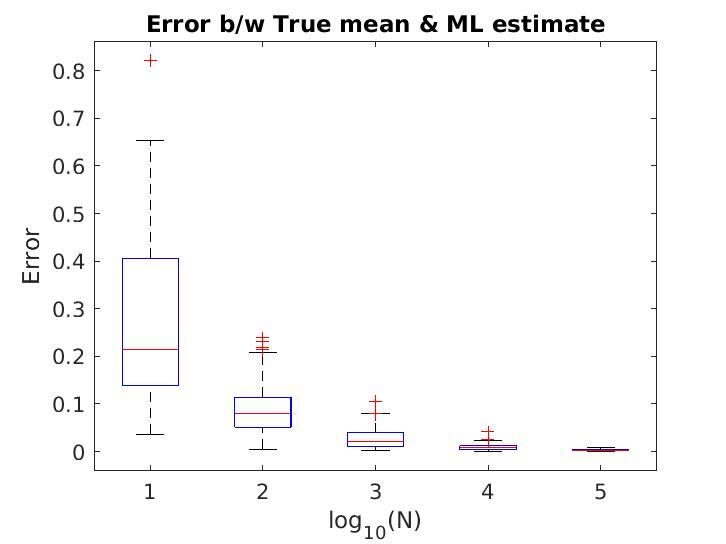
\includegraphics[scale=0.4]{q2/mean_err.jpg}
    \caption{Box plot of the error between the true mean $\mu$ and the ML estimate $\hat{\mu}_N$}
\end{figure}
\begin{figure}[H]
    \centering
    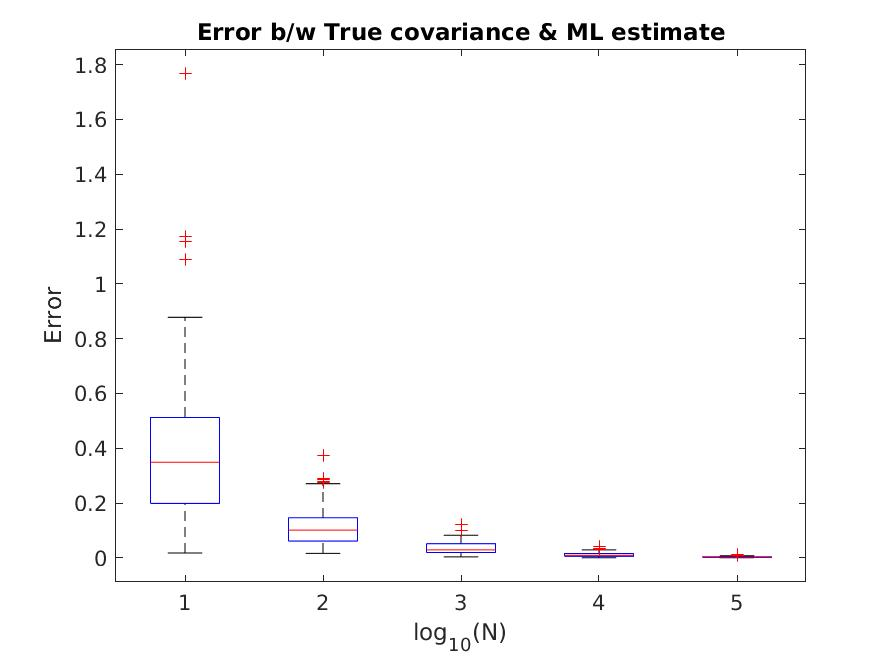
\includegraphics[scale=0.4]{q2/cov_err.jpg}
    \caption{Box plot of the error between the true covariance $C$ and the ML estimate $\hat{C}_N$}
\end{figure}

\subsection*{(d)}
From PCA, we know that principal mode of variation of data lies in the direction of the eigenvector corresponding to highest eigenvalue obtained on Eigen decomposition of the sample covariance matrix (here, \verb!cov_mle!). \\
Again, using \verb!eig! function we obtain the diagonal matrix \verb!lambda! whose diagonal elements are the eigenvalues. \\
As we only have two eigenvalues, a simple \verb!if-else! can be used to determine the principal mode of variation. \\
As we use sample mean (here, \verb!mean_mle!) to get the line and plot it using \verb!line!.
\begin{verbatim}
[Q, lambda] = eig(cov_mle);
if lambda(1, 1) > lambda(2, 2)
    ep = D(1,1)*Q(:, 1);
else
    ep = D(2,2)*Q(:, 2);
end
line([0 ep(1)] + mean_mle(1), [0 ep(2)] + mean_mle(2));
\end{verbatim}

Plots for N = {$10$, $10^2$, $10^3$, $10^4$, $10^5$}.
\begin{figure}[H]
    \centering
    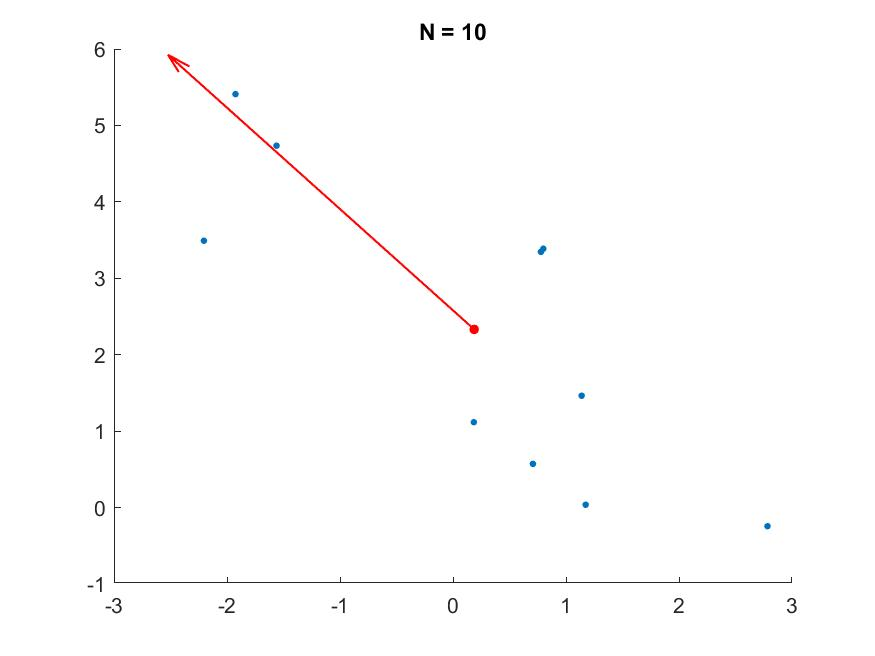
\includegraphics[scale=0.4]{q2/d_10.jpg}
    \caption{Scatter Plot for $N = 10$ with line showing principal mode of variation}
\end{figure}
\begin{figure}[H]
    \centering
    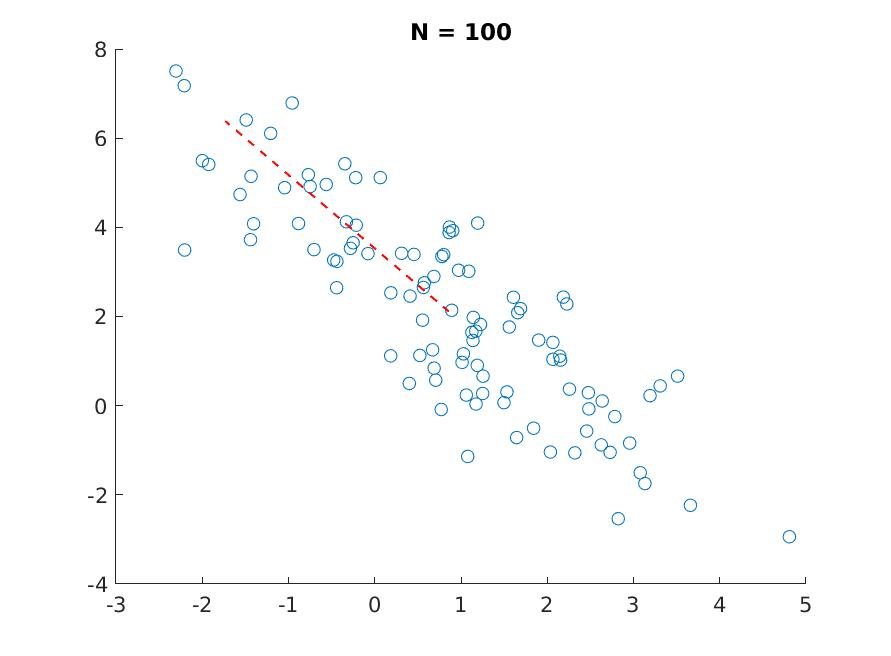
\includegraphics[scale=0.4]{q2/d_100.jpg}
    \caption{Scatter Plot for $N = 10^2$ with line showing principal mode of variation}
\end{figure}
\begin{figure}[H]
    \centering
    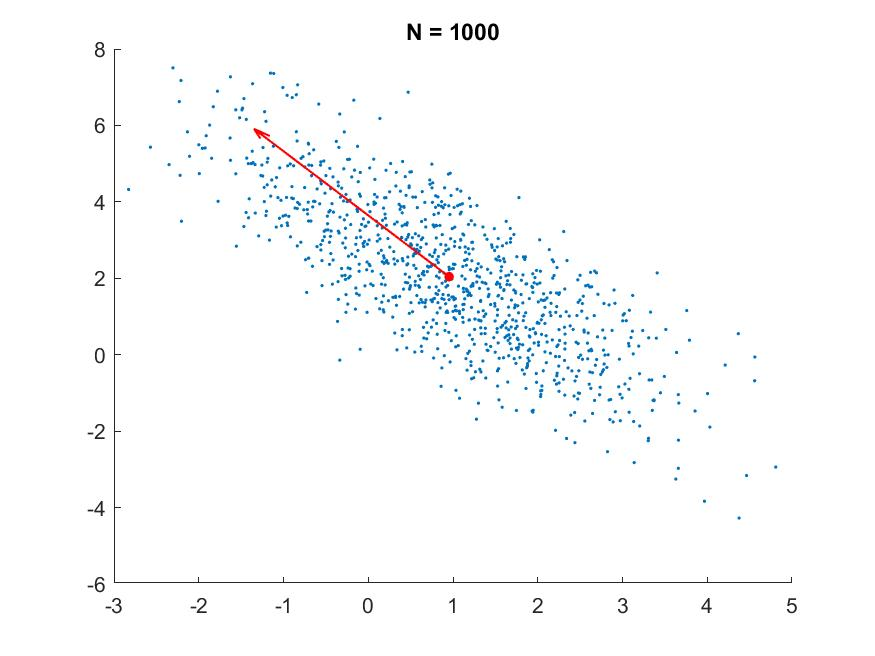
\includegraphics[scale=0.4]{q2/d_1000.jpg}
    \caption{Scatter Plot for $N = 10^3$ with line showing principal mode of variation}
\end{figure}
\begin{figure}[H]
    \centering
    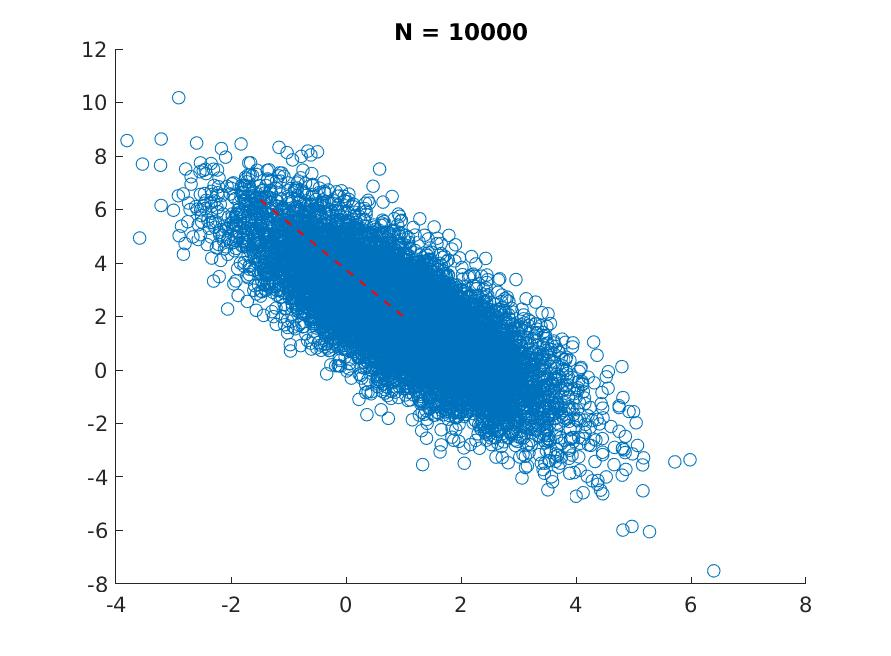
\includegraphics[scale=0.4]{q2/d_10000.jpg}
    \caption{Scatter Plot for $N = 10^4$ with line showing principal mode of variation}
\end{figure}
\begin{figure}[H]
    \centering
    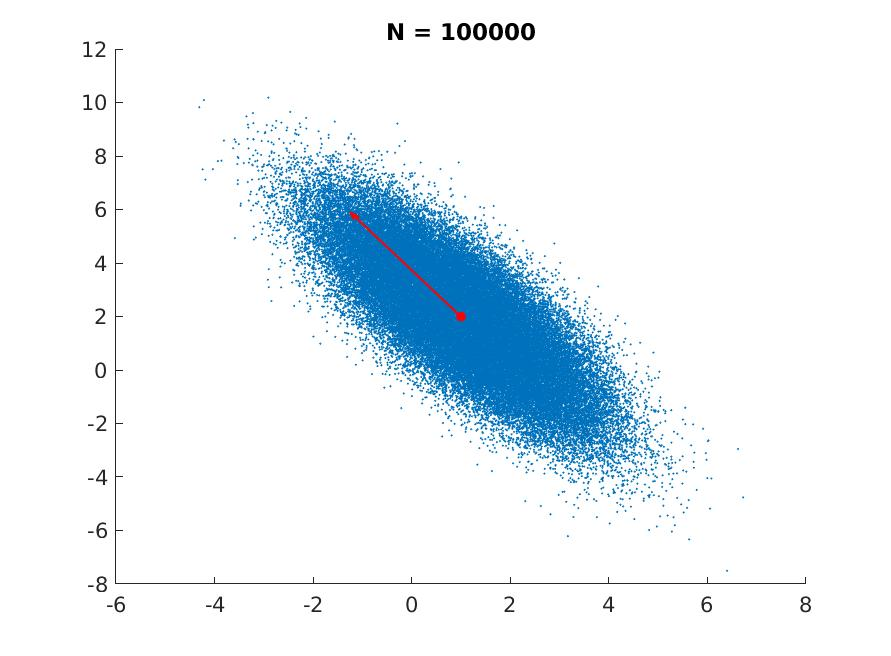
\includegraphics[scale=0.4]{q2/d_100000.jpg}
    \caption{Scatter Plot for $N = 10^5$ with line showing principal mode of variation}
\end{figure}





\newpage
\section*{Question 3}
\addcontentsline{toc}{section}{Question 3}
\setcounter{equation}{0}
\setcounter{figure}{0}
We have been given observed set of data $\{ \mathbf{z}_i \}_{i=1}^{N}$, where $\mathbf{z}_i = (x_i, y_i)$\\
We need to find a linear relationship between the RVs $X$ and $Y$

\medskip
Thus, we need to find $m, c$ such that $Y \approx mX + c$ using PCA.\\
This is essentially dimensionality reduction from $\mathbb{R}^2$ to $\mathbb{R}$\\
Thus, we need to find the first principal mode of variance/principal component of $\{ \mathbf{z}_i \}_{i=1}^{N}$

\medskip
Let the sample mean be $\mu = \bigg(\mu_1 = \frac{\sum_{i=1}^{N}x_i}{N},\  \mu_2 = \frac{\sum_{i=1}^{N}y_i}{N}\bigg)$, then first we center the data about $\mu$.\\
Let the sample covariance matrix of the new centered data be $C$.\\
Since we are not allowed to use \texttt{cov()} and \texttt{mean()}, we compute the sample $\mu = \frac{\sum_{i=1}^{N}\mathbf{z_i}}{N}$.\\
Let $Z = [\mathbf{z_i} - \mu]$ be a $N\times2$ matrix of the entire \textbf{mean-centered} observed data.\\
Then $C = \frac{Z^T Z}{N-1}$ will give us the covariance matrix.

\medskip
On eigenvalue decomposition of $C$, we get $C = Q\Lambda Q^T$, let $\mathbf{d}$ correspond to the diagonal values of $\Lambda$, let $j = \text{argmax}_{i: 1\le i\le 2} \ \mathbf{d}$, then the $j^{th}$ column of Q corresponds to the principal mode of variation, $\mathbf{v} = (v_1, v_2)$

\medskip
Thus, $m = \frac{v_2}{v_1}$, and $y = mx$, since this was the centered coordinate system (about $\mu$), we need to shift back to the original coordinate system, thus, the final straight line will be $y-\mu_2 = m(x - \mu_1)$

\medskip
The same method as above has been implemented in \texttt{q3.m}

\medskip
In this case, PCA chooses the direction along which the variance of the projected data is maximized.\\
The quality of the approximation worsens with the given data deviating from a linear relationship (when we want to fit a straight line through the data).\\
In the worst case, consider the data distributed around a circle.\\
In this case, all the directions through the mean will have approximately the same variance of the projected data, thus there is no ``best" direction.\\
In the first case, there appears to be a linear relationship in the given data, thus reducing the dimension to 1 using PCA yields good quality results.\\
In the second case, the data is distributed in an approximate ellipse, thus the major axis will be the direction which maximizes the variance of the projected data, however, in case of an ellipse, there is considerable variance along the minor axis too, PCA approximation loses this information about the original data and thus the quality of results is poor compared to the first set of data.\\
Thus, trying to reduce the dimension of the data to 1, in data which varies along more than one direction is thus meaningless in most of the cases.

\subsection*{Instructions for running the code:}
\begin{enumerate}[itemsep=-1ex]
    \item Unzip and \texttt{cd} to \texttt{code}, under this find the file named \texttt{q3.m}
    \item Find the variable \texttt{PATH\_TO\_LOAD} on the $7^{th}$ line, change this to \texttt{DATA\_PATH\_1} or \texttt{DATA\_PATH\_2} accordingly, run the file, a scatter plot with a fitted line will generated and saved to the \texttt{plots} folder.
\end{enumerate}

\newpage
\section*{Question 4}
\addcontentsline{toc}{section}{Question 4}
\setcounter{equation}{0}
\setcounter{figure}{0}

First, we extract the images of handwritten digits from dataset \verb!"mnist.mat"! and recast the training data into double and normalize it. \\
Normalization helps to reduce errors which otherwise occur due to high range of values in covariance matrix. \\
We also reshape the images into a vector for ease of computation.
\begin{verbatim}
DATA_PATH = "../data/mnist.mat";
load(DATA_PATH, "-mat"); % Load data
N = length(digits_train);
WIDTH = size(digits_train, 1);
SIZE = WIDTH^2;
% Reshape, Recast, Normalize image intensity
train_data = cast(reshape(digits_train, [SIZE N]), 'double')/255;
\end{verbatim}

Now, we have to tasks ahead, to find the mean and covariance and then find the principal mode of variations (eigenvectors of covariance matrix).
\begin{verbatim}
count = sum(labels_train==digit);
digit_data = train_data(:, labels_train == digit);
mean = sum(digit_data, 2)/count; % sample mean
cov = (digit_data-mean)*(digit_data'-mean')/(count-1); % sample cov
\end{verbatim}
The above code snippet is inside a for loop iterating over \verb!digit! which stores the digit we are working on. \\
First, we \verb!count! the number of images (N) of the digit in the training data and then find sample mean $\mu = \sum_{i=1}^N x_i / N$ and sample covariance $C = \sum_{i=1}^N (x_i - \mu) (x_i - \mu)^T / (N - 1)$. \\

Next, we use \verb!eig! function for Eigen Decomposition of the covariance matrix.
\begin{verbatim}
[Q, D] = eig(cov);
dia = diag(D); % Get the diagonals elements as a vector

% Find the highest eigenvalue and its corresponding eigenvector
[lamb1, index1] = max(dia);
v1 = Q(:,index1);

% Sort the eigenvalues to analyse their distribution
dia = sort(dia,'descend');
dia(dia<0)=0; % Fixing precision error due to eig()
\end{verbatim}
It was observed that \verb!eig! returned eigenvalues like $-10^{-10}$, which we know is only precision error as eigenvalues of a Positive semi-definite matrix are non-negative. \\

We plot the sorted eigenvalues (784 in total) and we observe a sudden dip very soon. To further analyse, we plot it with log scale on X-axis and observe that by the time we reach 10, the values have fallen to less than 20\% of highest value (located at 1) for all digits. \\
For some digits (especially 1), the decrease is more drastic than others.

We compute the number of eigenvalues having value more than 1\% of the highest value and here is the result. (Also printed on Console in MATLAB)
\begin{verbatim}
56 Significant modes of variation for Digit 0 (Number of Eigenvalues > 1% of Max Eigenvalue)
27 Significant modes of variation for Digit 1 (Number of Eigenvalues > 1% of Max Eigenvalue)
86 Significant modes of variation for Digit 2 (Number of Eigenvalues > 1% of Max Eigenvalue)
86 Significant modes of variation for Digit 3 (Number of Eigenvalues > 1% of Max Eigenvalue)
83 Significant modes of variation for Digit 4 (Number of Eigenvalues > 1% of Max Eigenvalue)
69 Significant modes of variation for Digit 5 (Number of Eigenvalues > 1% of Max Eigenvalue)
60 Significant modes of variation for Digit 6 (Number of Eigenvalues > 1% of Max Eigenvalue)
63 Significant modes of variation for Digit 7 (Number of Eigenvalues > 1% of Max Eigenvalue)
89 Significant modes of variation for Digit 8 (Number of Eigenvalues > 1% of Max Eigenvalue)
63 Significant modes of variation for Digit 9 (Number of Eigenvalues > 1% of Max Eigenvalue)
\end{verbatim}

The observed values are far less than $28^2 = 784$. \\
One of the many obvious reason is the consistent background. There are several pixels in the background which are more or less left untouched by the person drawing the digits. \\
Another reason is that it is a common knowledge on how to draw a given digit and so the human-error is not prominent either. \\ 

For the next part, we use the calculated principal mode of variation \verb!v1! and it corresponding eigenvalue \verb!lambda1! to draw\footnote{I have used \texttt{pbaspect([1 1 1])} in place of suggested \texttt{axis equal}, here both are equivalent as range of both axes is (1,28)} the 3 images of form: $\mu - \sqrt{\lambda_1}v_1$, $\mu$ and $\mu + \sqrt{\lambda_1}v_1$. \\
In all digits except 0 and 2, we observe that the three images mostly differ by rotation of the digit. \\
In digit 0, in addition to the difference in rotation, we also observe some circular to elliptical transform (compressing along the horizontal axis). \\
In digit 2, we observe that the lobe at the bottom turn while drawing digit varies in size along with a observable rotation (though less significant)

For digit 1, the principal mode of variation tells that people write 1 more like a straight line which maybe slanted (forward slash). Maximum variation is observed in angle of the line. 

\newpage
\begin{figure}[H]
    \begin{floatrow}
        \ffigbox[0.45\textwidth]{}
        {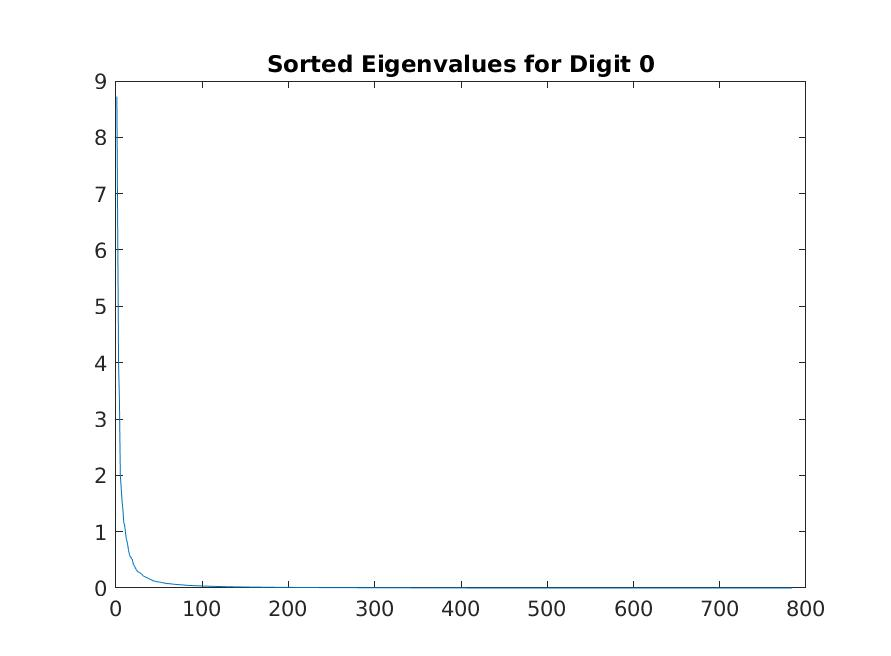
\includegraphics[height=0.35\textwidth]{q4/eigenvalues_0.jpg}}
        \ffigbox[0.45\textwidth]{}
        {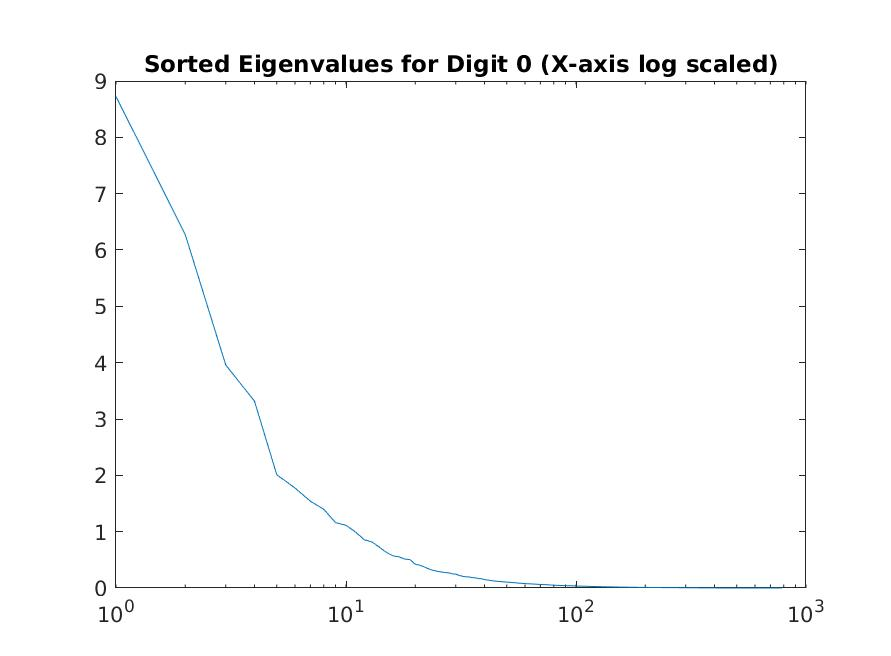
\includegraphics[height=0.35\textwidth]{q4/eigenvalues_log_0.jpg}}
    \end{floatrow}
    \vspace{1em}
    \begin{floatrow}
        \ffigbox[0.9\textwidth]{}
        {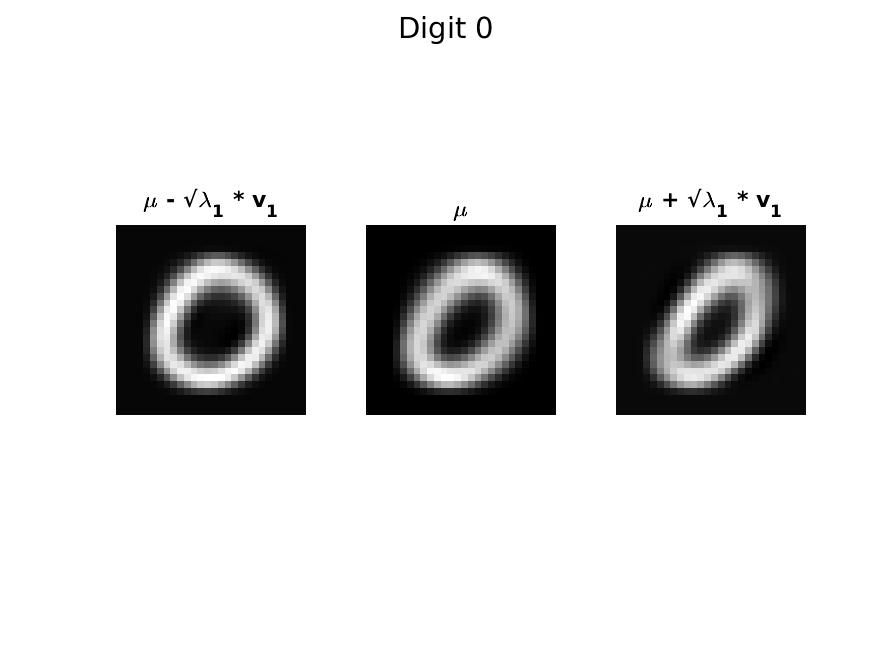
\includegraphics[height=0.7\textwidth]{q4/trip_img_0.jpg}}
    \end{floatrow}
\end{figure}
\newpage
\begin{figure}[H]
    \begin{floatrow}
        \ffigbox[0.45\textwidth]{}
        {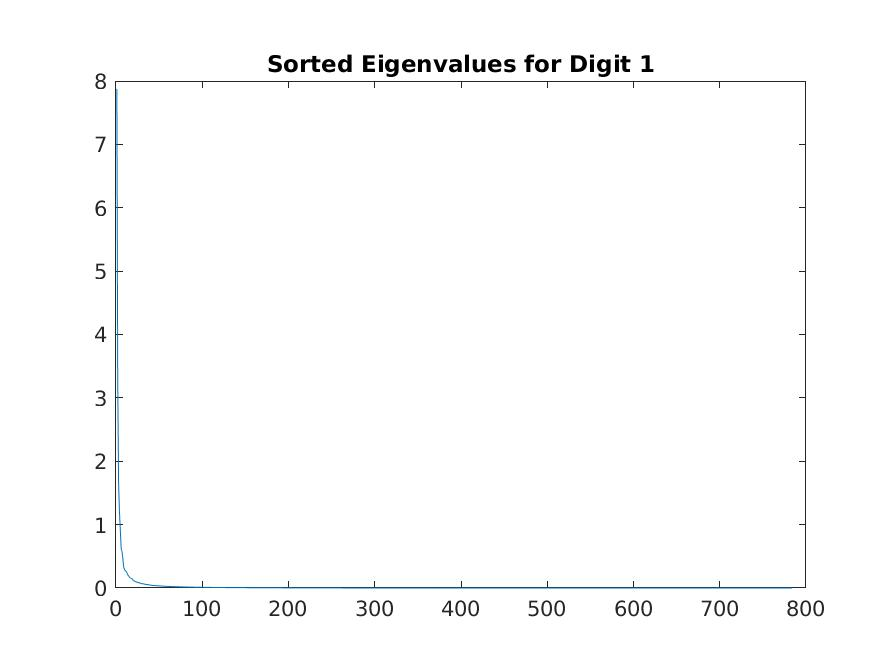
\includegraphics[height=0.35\textwidth]{q4/eigenvalues_1.jpg}}
        \ffigbox[0.45\textwidth]{}
        {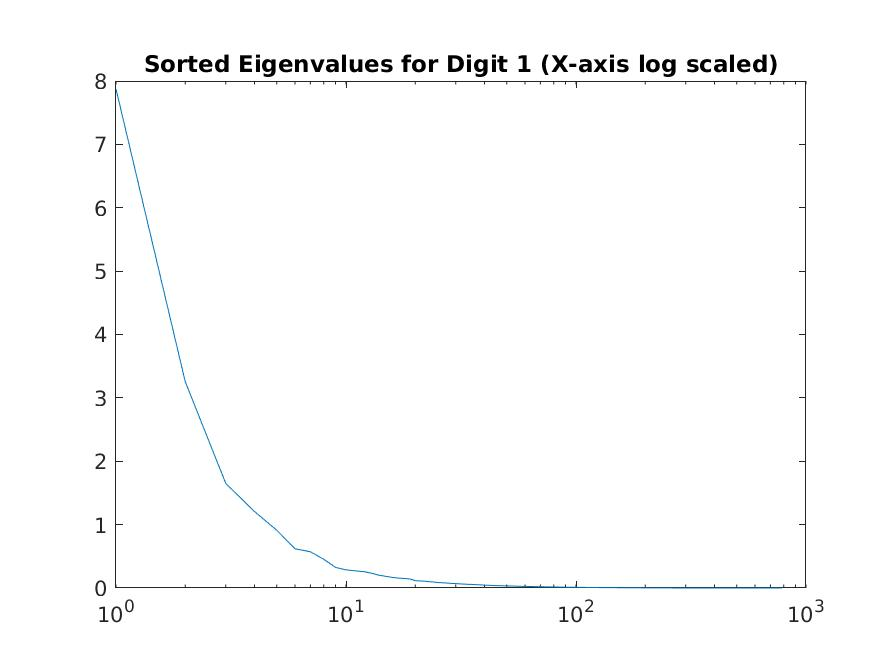
\includegraphics[height=0.35\textwidth]{q4/eigenvalues_log_1.jpg}}
    \end{floatrow}
    \vspace{1em}
    \begin{floatrow}
        \ffigbox[0.9\textwidth]{}
        {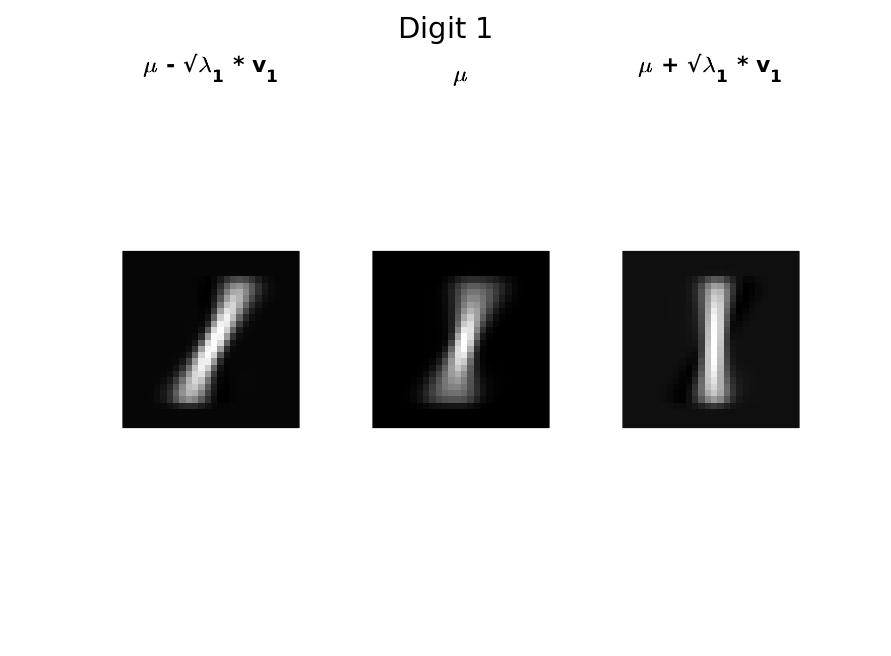
\includegraphics[height=0.7\textwidth]{q4/trip_img_1.jpg}}
    \end{floatrow}
\end{figure}
\newpage
\begin{figure}[H]
    \begin{floatrow}
        \ffigbox[0.45\textwidth]{}
        {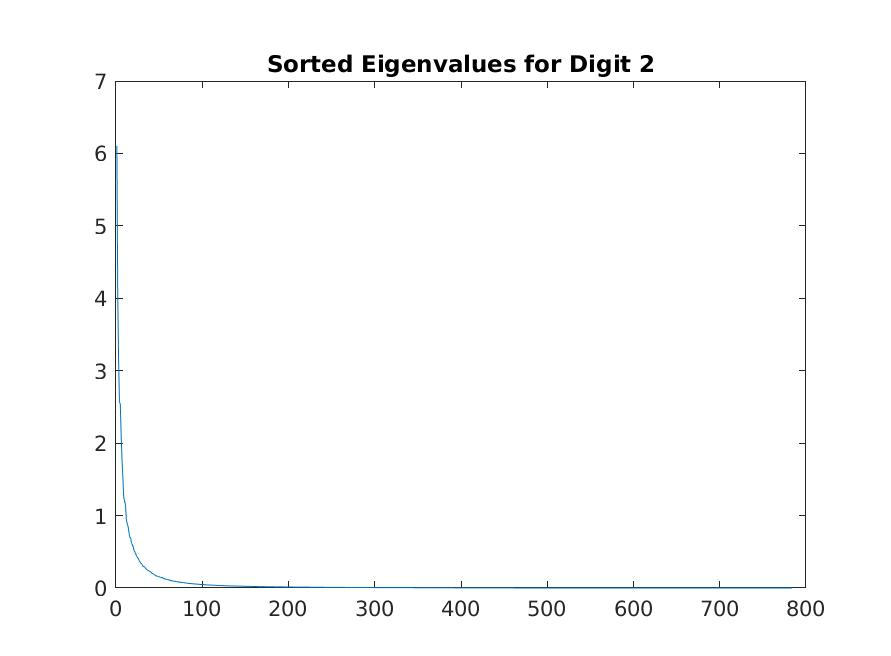
\includegraphics[height=0.35\textwidth]{q4/eigenvalues_2.jpg}}
        \ffigbox[0.45\textwidth]{}
        {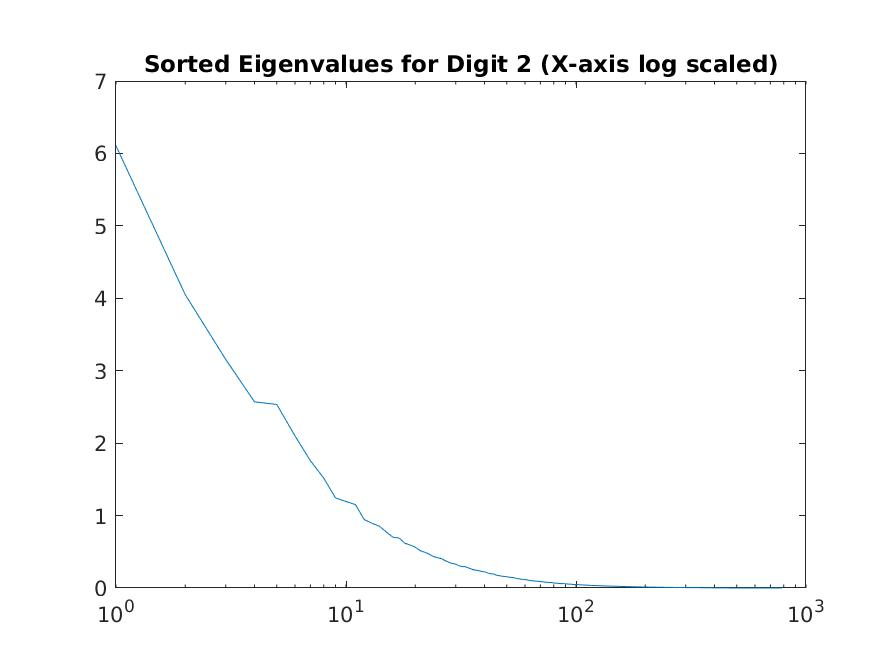
\includegraphics[height=0.35\textwidth]{q4/eigenvalues_log_2.jpg}}
    \end{floatrow}
    \vspace{1em}
    \begin{floatrow}
        \ffigbox[0.9\textwidth]{}
        {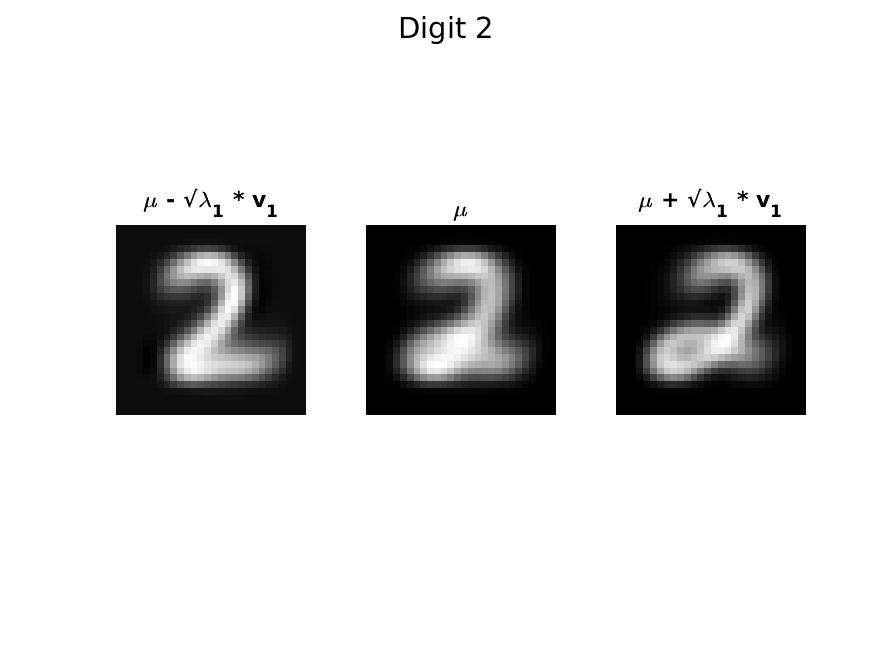
\includegraphics[height=0.7\textwidth]{q4/trip_img_2.jpg}}
    \end{floatrow}
\end{figure}
\newpage
\begin{figure}[H]
    \begin{floatrow}
        \ffigbox[0.45\textwidth]{}
        {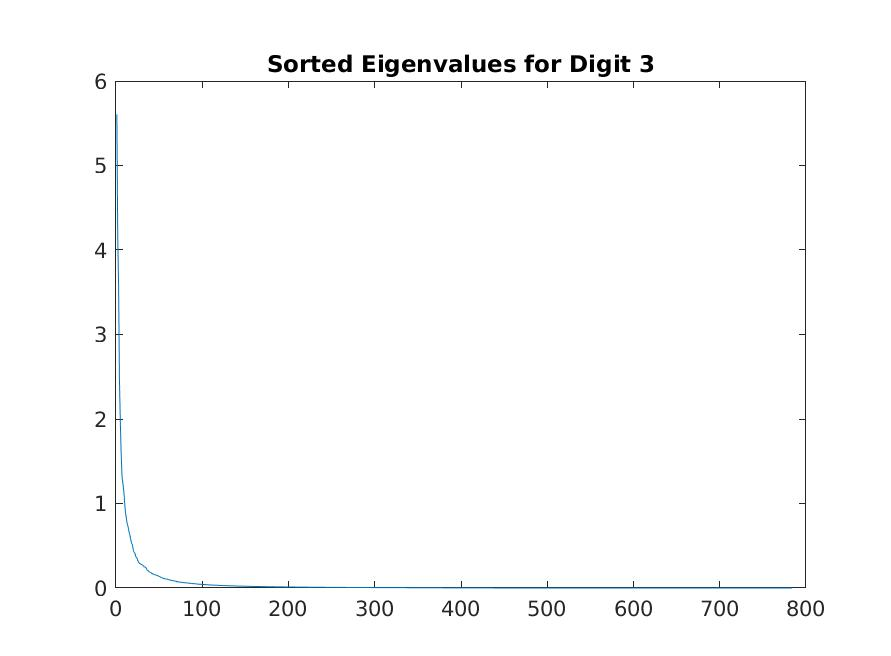
\includegraphics[height=0.35\textwidth]{q4/eigenvalues_3.jpg}}
        \ffigbox[0.45\textwidth]{}
        {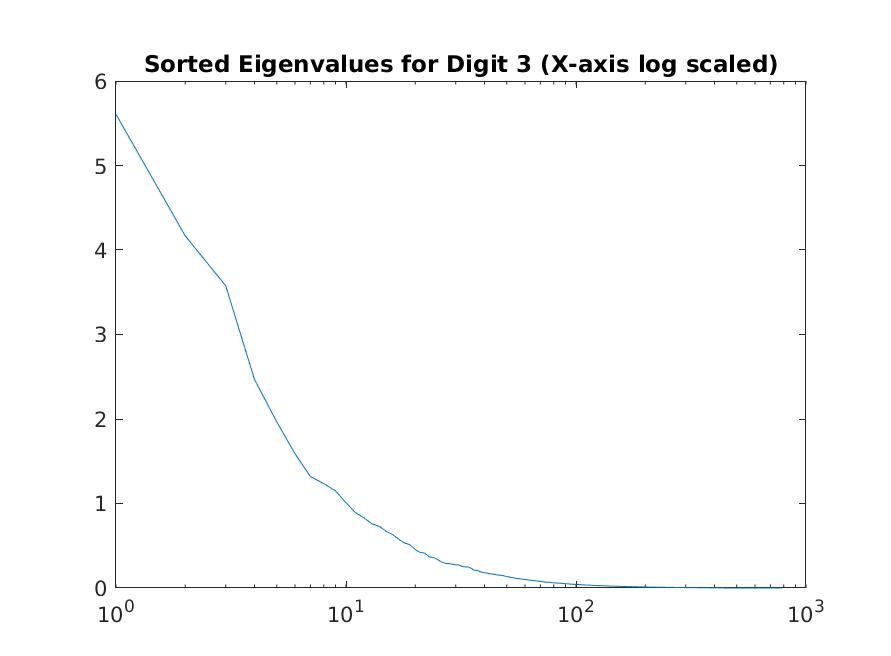
\includegraphics[height=0.35\textwidth]{q4/eigenvalues_log_3.jpg}}
    \end{floatrow}
    \vspace{1em}
    \begin{floatrow}
        \ffigbox[0.9\textwidth]{}
        {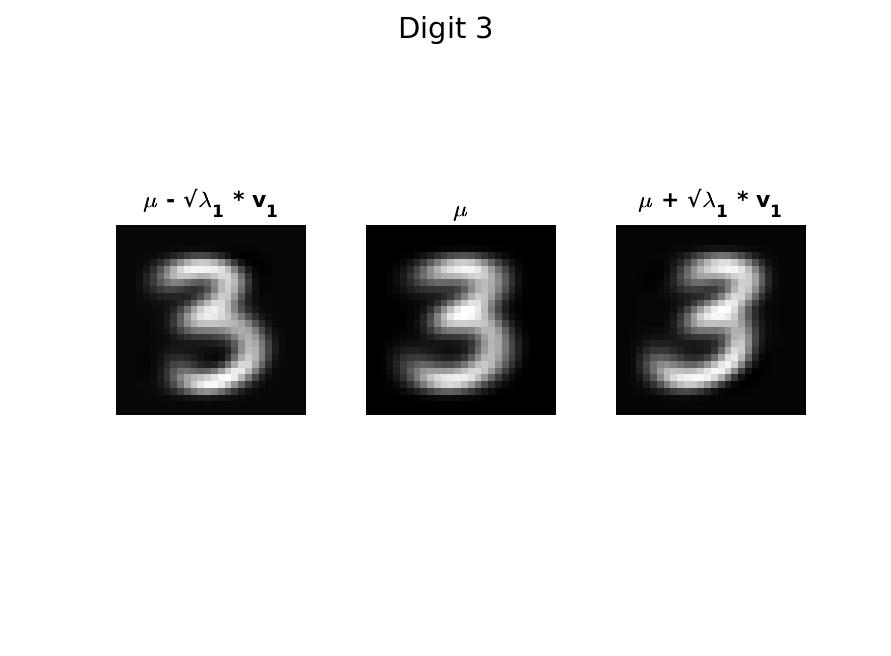
\includegraphics[height=0.7\textwidth]{q4/trip_img_3.jpg}}
    \end{floatrow}
\end{figure}
\newpage
\begin{figure}[H]
    \begin{floatrow}
        \ffigbox[0.45\textwidth]{}
        {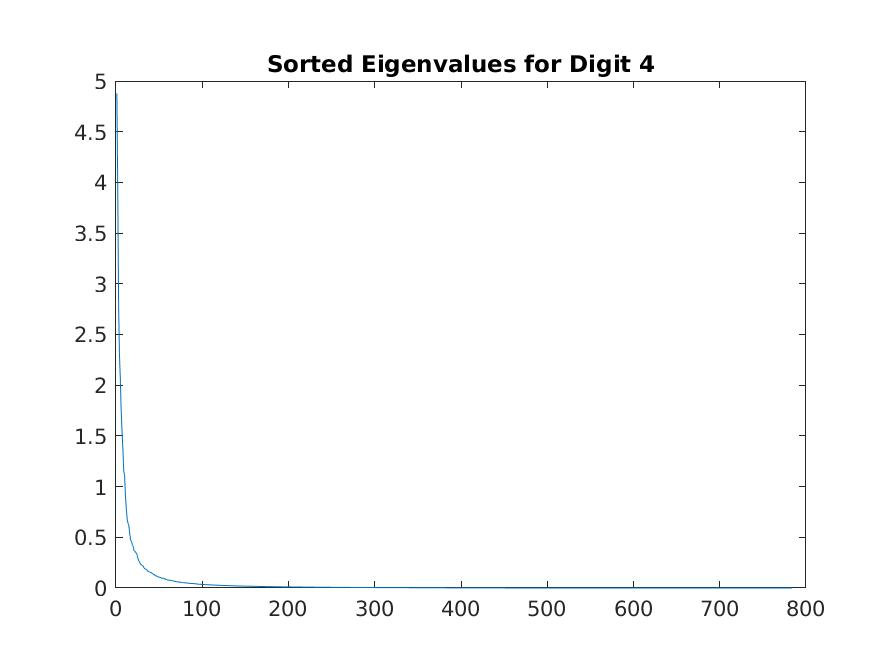
\includegraphics[height=0.35\textwidth]{q4/eigenvalues_4.jpg}}
        \ffigbox[0.45\textwidth]{}
        {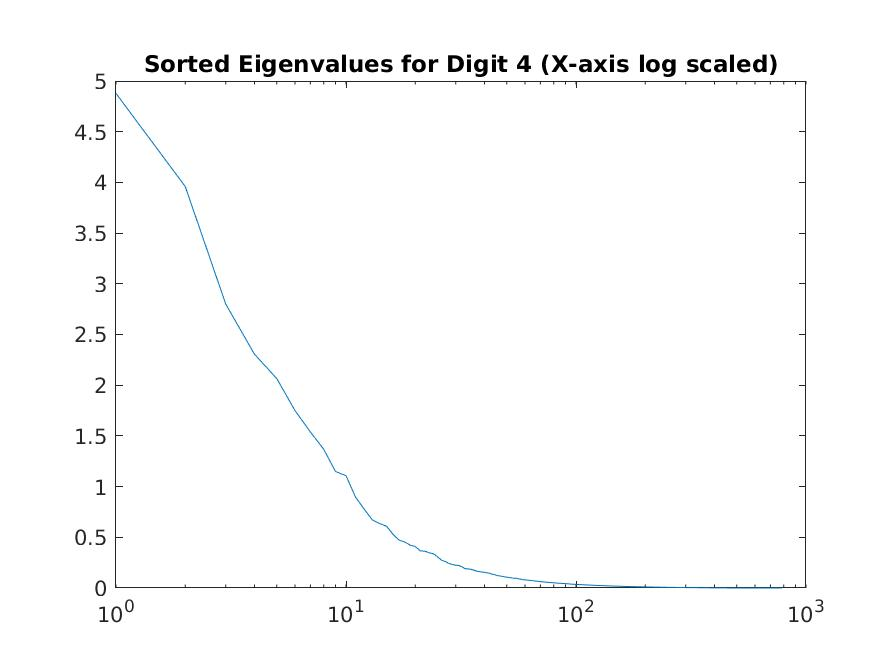
\includegraphics[height=0.35\textwidth]{q4/eigenvalues_log_4.jpg}}
    \end{floatrow}
    \vspace{1em}
    \begin{floatrow}
        \ffigbox[0.9\textwidth]{}
        {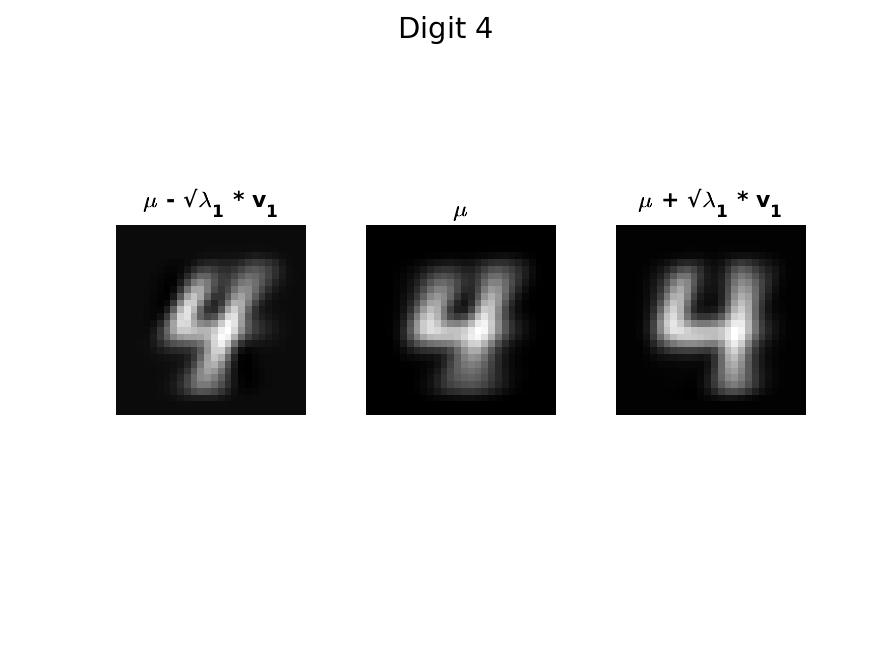
\includegraphics[height=0.7\textwidth]{q4/trip_img_4.jpg}}
    \end{floatrow}
\end{figure}
\newpage
\begin{figure}[H]
    \begin{floatrow}
        \ffigbox[0.45\textwidth]{}
        {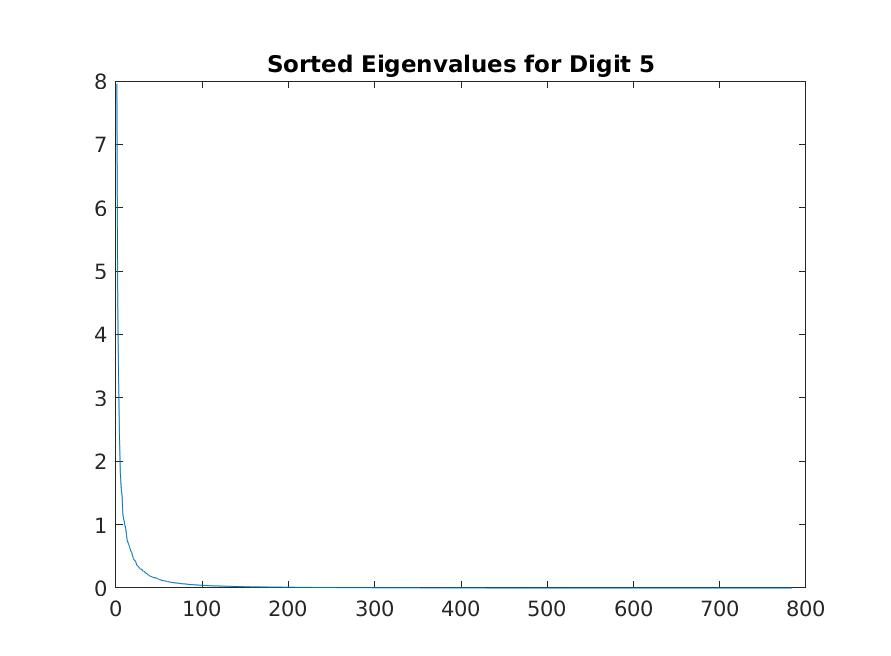
\includegraphics[height=0.35\textwidth]{q4/eigenvalues_5.jpg}}
        \ffigbox[0.45\textwidth]{}
        {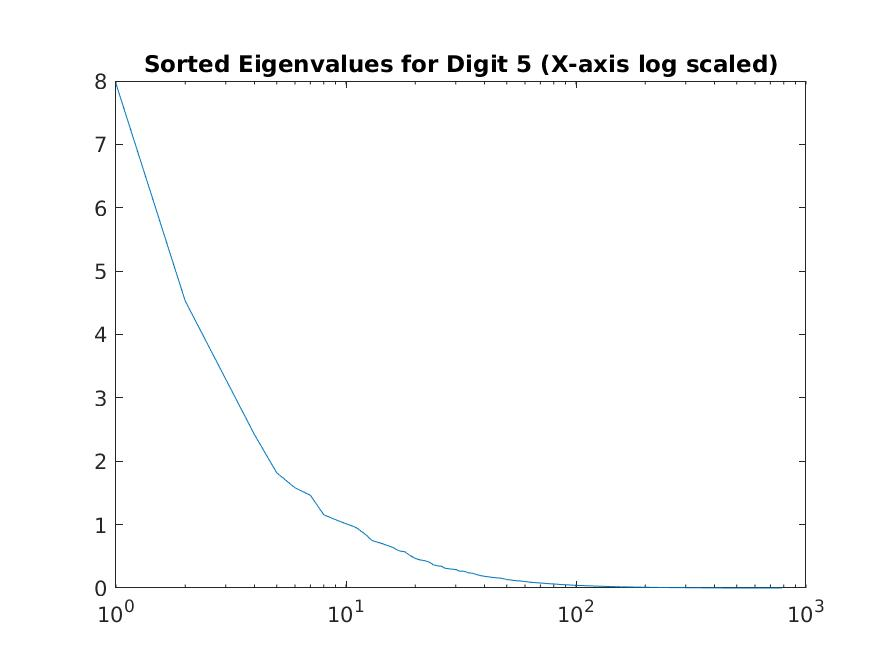
\includegraphics[height=0.35\textwidth]{q4/eigenvalues_log_5.jpg}}
    \end{floatrow}
    \vspace{1em}
    \begin{floatrow}
        \ffigbox[0.9\textwidth]{}
        {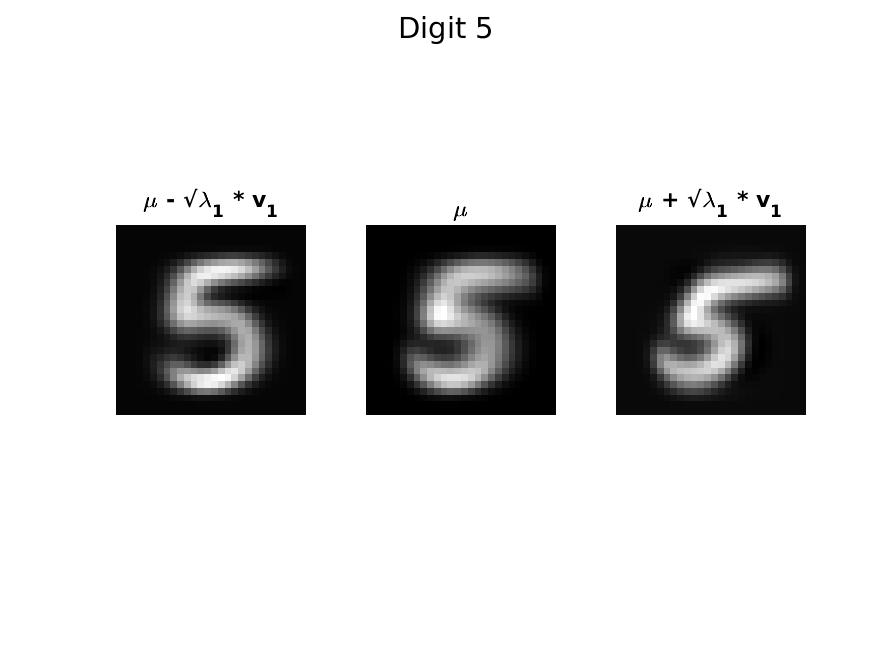
\includegraphics[height=0.7\textwidth]{q4/trip_img_5.jpg}}
    \end{floatrow}
\end{figure}
\newpage
\begin{figure}[H]
    \begin{floatrow}
        \ffigbox[0.45\textwidth]{}
        {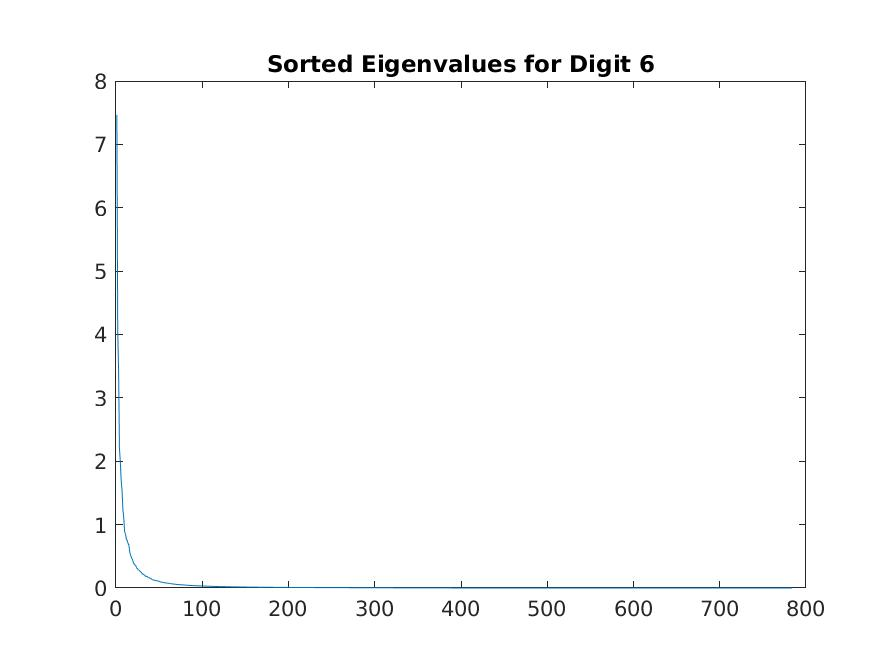
\includegraphics[height=0.35\textwidth]{q4/eigenvalues_6.jpg}}
        \ffigbox[0.45\textwidth]{}
        {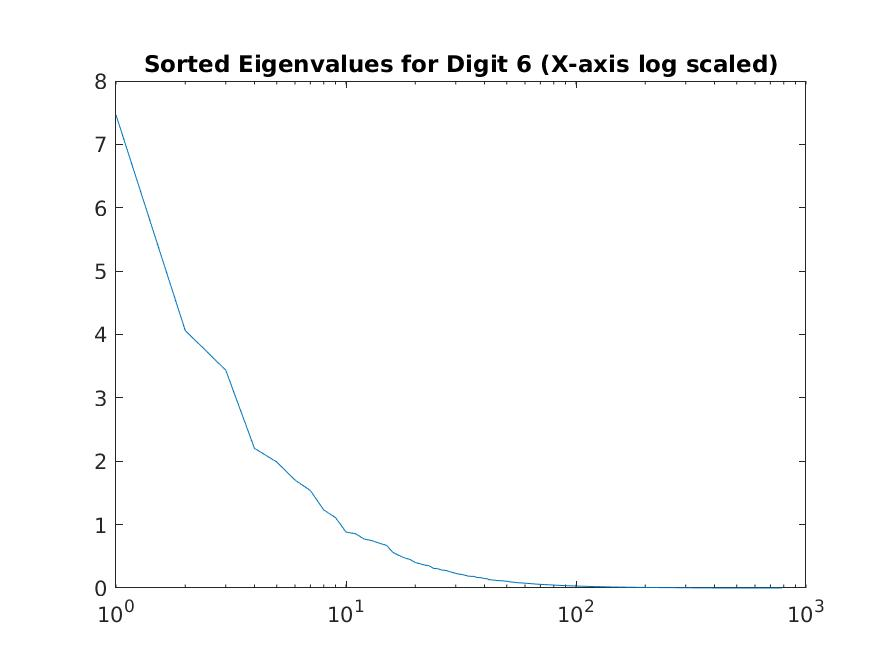
\includegraphics[height=0.35\textwidth]{q4/eigenvalues_log_6.jpg}}
    \end{floatrow}
    \vspace{1em}
    \begin{floatrow}
        \ffigbox[0.9\textwidth]{}
        {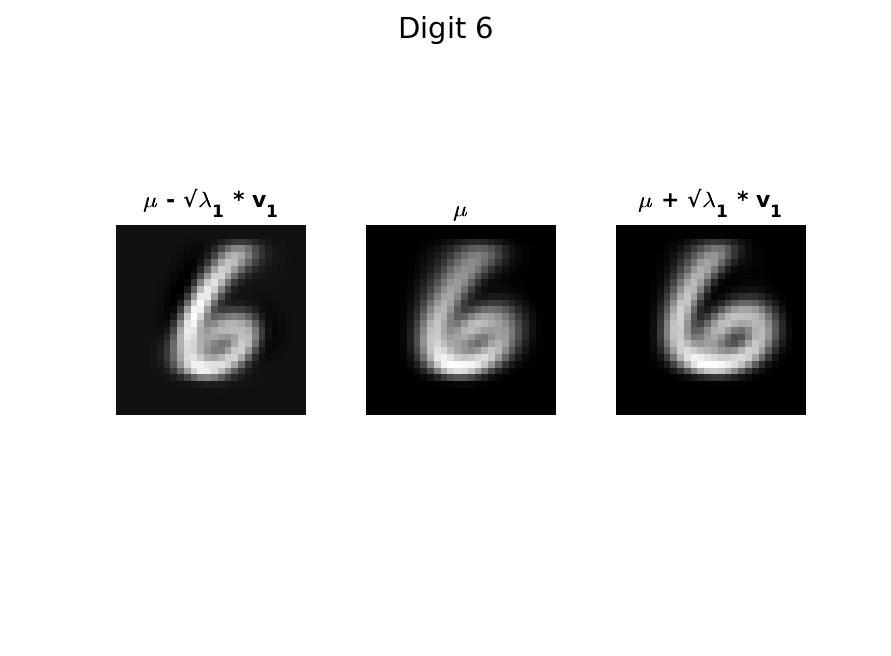
\includegraphics[height=0.7\textwidth]{q4/trip_img_6.jpg}}
    \end{floatrow}
\end{figure}
\newpage
\begin{figure}[H]
    \begin{floatrow}
        \ffigbox[0.45\textwidth]{}
        {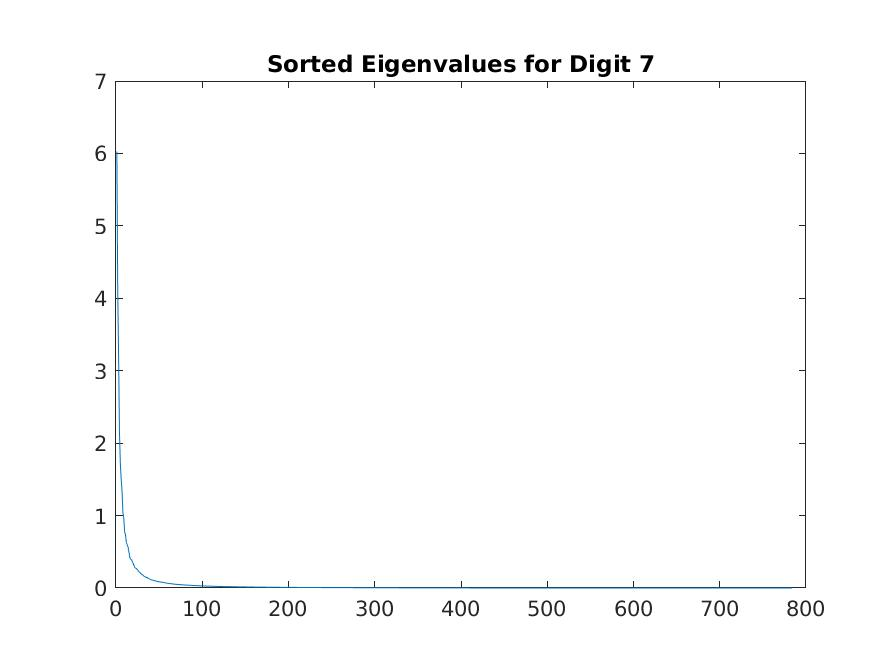
\includegraphics[height=0.35\textwidth]{q4/eigenvalues_7.jpg}}
        \ffigbox[0.45\textwidth]{}
        {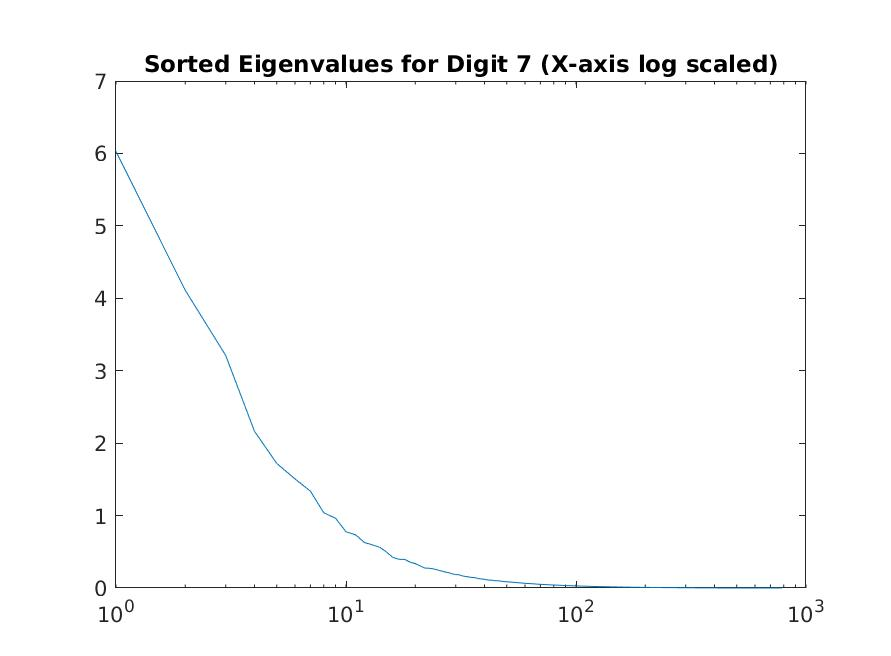
\includegraphics[height=0.35\textwidth]{q4/eigenvalues_log_7.jpg}}
    \end{floatrow}
    \vspace{1em}
    \begin{floatrow}
        \ffigbox[0.9\textwidth]{}
        {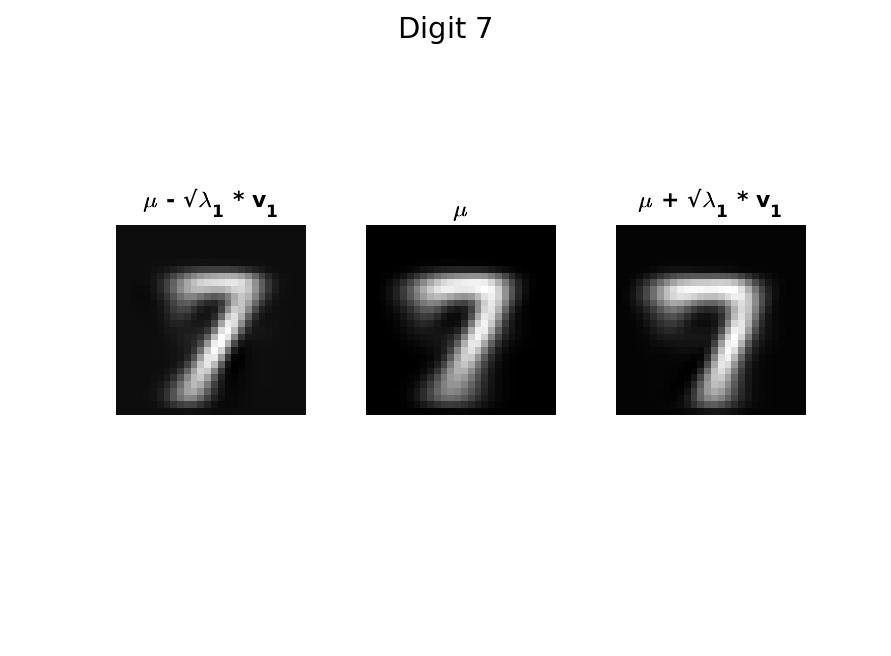
\includegraphics[height=0.7\textwidth]{q4/trip_img_7.jpg}}
    \end{floatrow}
\end{figure}
\newpage
\begin{figure}[H]
    \begin{floatrow}
        \ffigbox[0.45\textwidth]{}
        {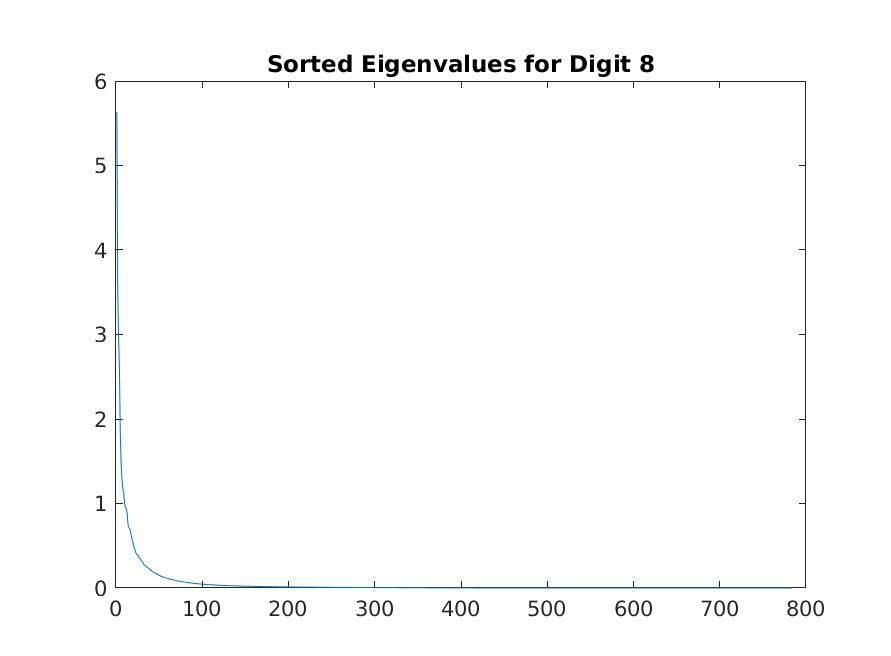
\includegraphics[height=0.35\textwidth]{q4/eigenvalues_8.jpg}}
        \ffigbox[0.45\textwidth]{}
        {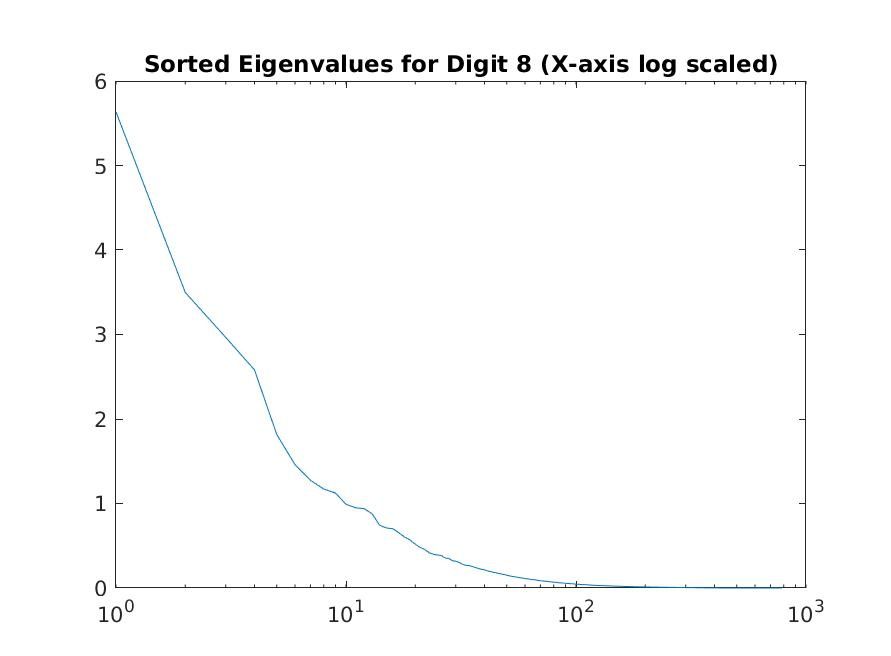
\includegraphics[height=0.35\textwidth]{q4/eigenvalues_log_8.jpg}}
    \end{floatrow}
    \vspace{1em}
    \begin{floatrow}
        \ffigbox[0.9\textwidth]{}
        {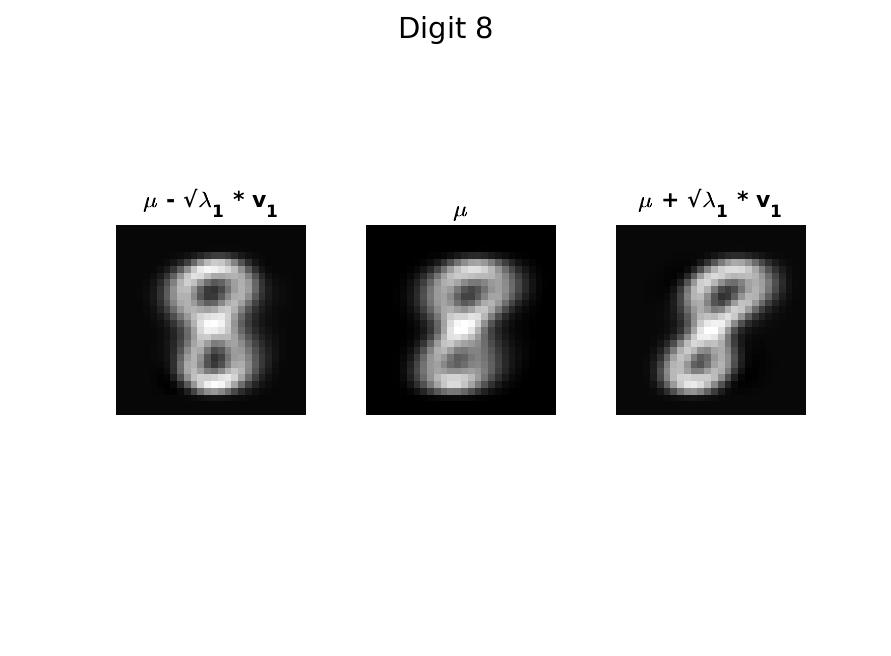
\includegraphics[height=0.7\textwidth]{q4/trip_img_8.jpg}}
    \end{floatrow}
\end{figure}
\newpage
\begin{figure}[H]
    \begin{floatrow}
        \ffigbox[0.45\textwidth]{}
        {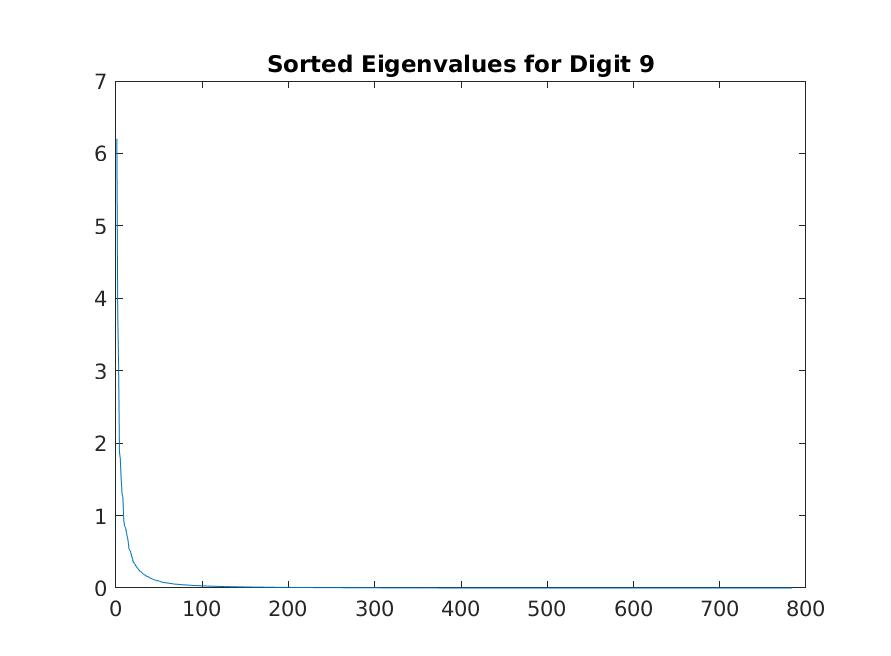
\includegraphics[height=0.35\textwidth]{q4/eigenvalues_9.jpg}}
        \ffigbox[0.45\textwidth]{}
        {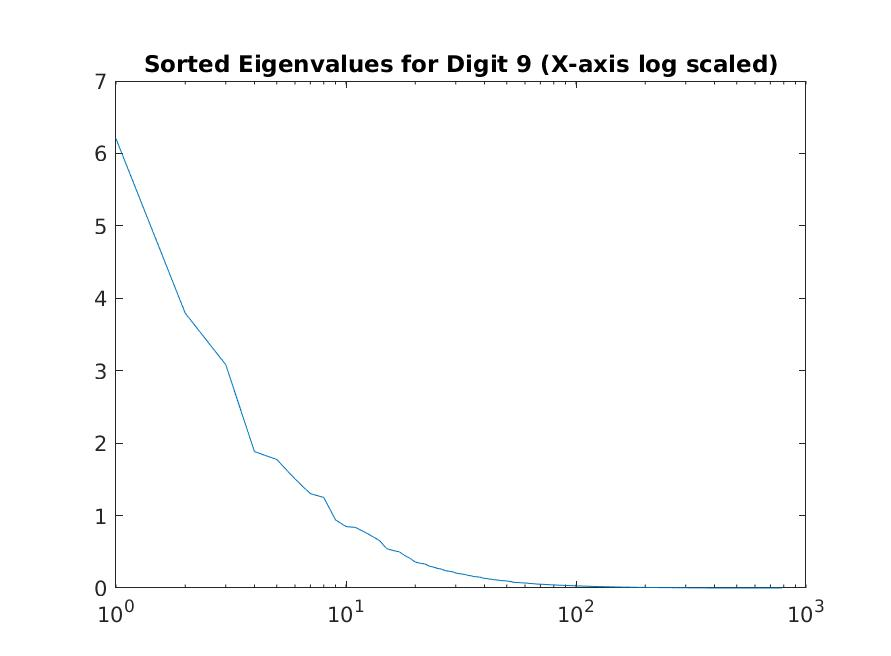
\includegraphics[height=0.35\textwidth]{q4/eigenvalues_log_9.jpg}}
    \end{floatrow}
    \vspace{1em}
    \begin{floatrow}
        \ffigbox[0.9\textwidth]{}
        {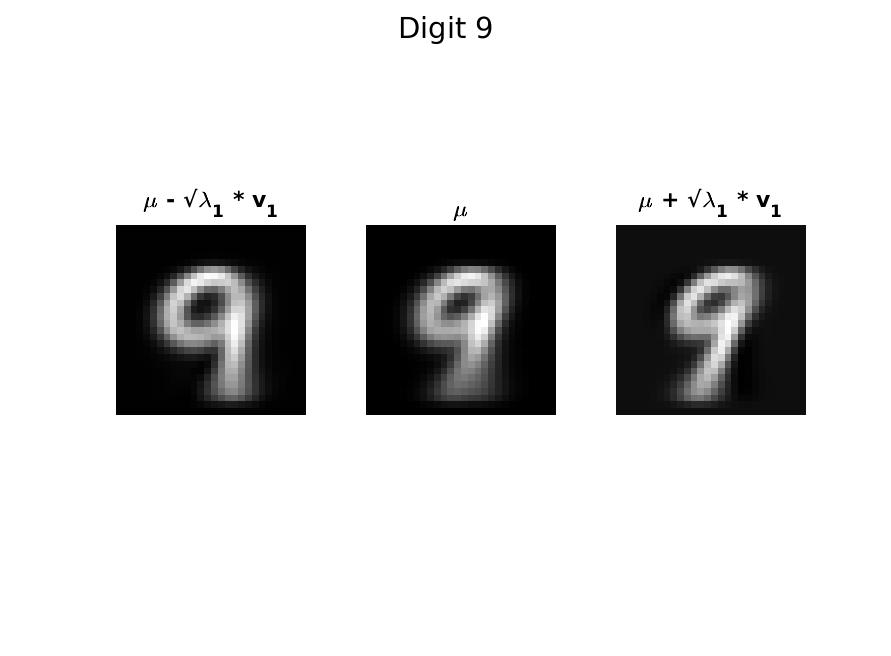
\includegraphics[height=0.7\textwidth]{q4/trip_img_9.jpg}}
    \end{floatrow}
\end{figure}

\newpage
\section*{Question 5}
\addcontentsline{toc}{section}{Question 5}
\setcounter{equation}{0}
\setcounter{figure}{0}
We continue with approach explained Question 4 for extracting the data and calculating sample mean and sample covariance.


\begin{figure}[H]
    \begin{floatrow}
        \ffigbox[0.47\textwidth]{}
        {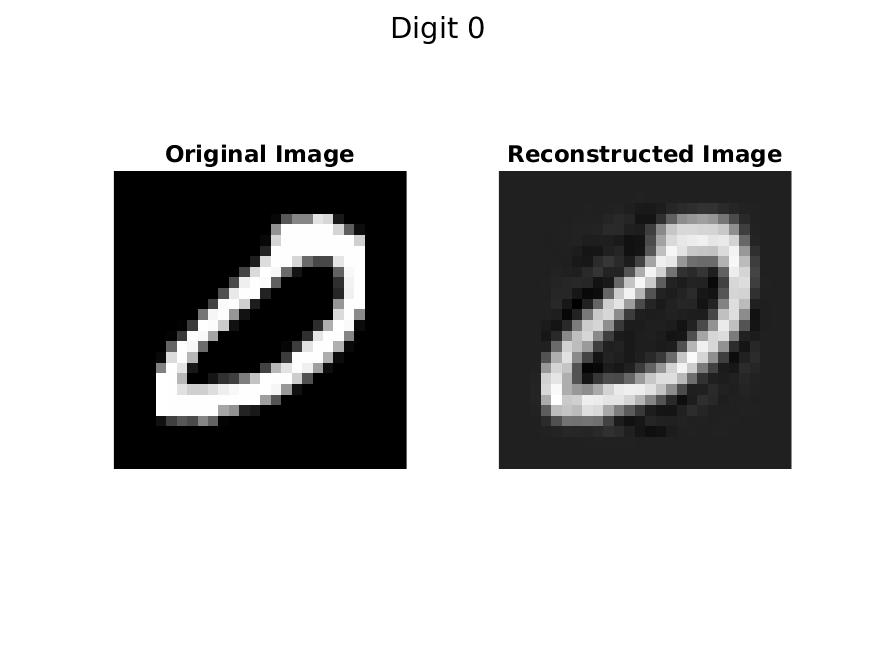
\includegraphics[height=0.40\textwidth]{q5/comp_0.jpg}}
        \ffigbox[0.47\textwidth]{}
        {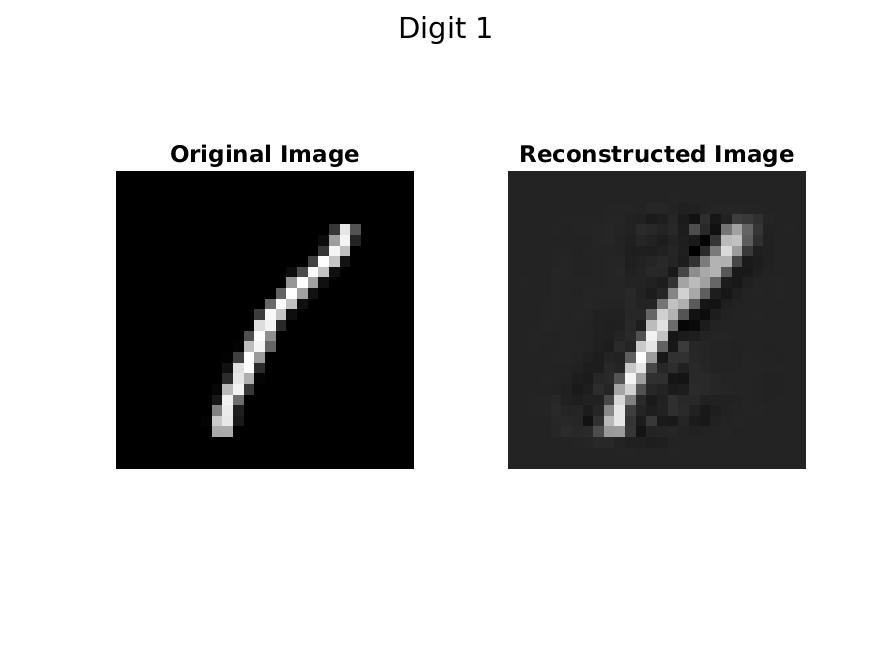
\includegraphics[height=0.40\textwidth]{q5/comp_1.jpg}}
    \end{floatrow}
\end{figure}
\begin{figure}[H]
    \begin{floatrow}
        \ffigbox[0.47\textwidth]{}
        {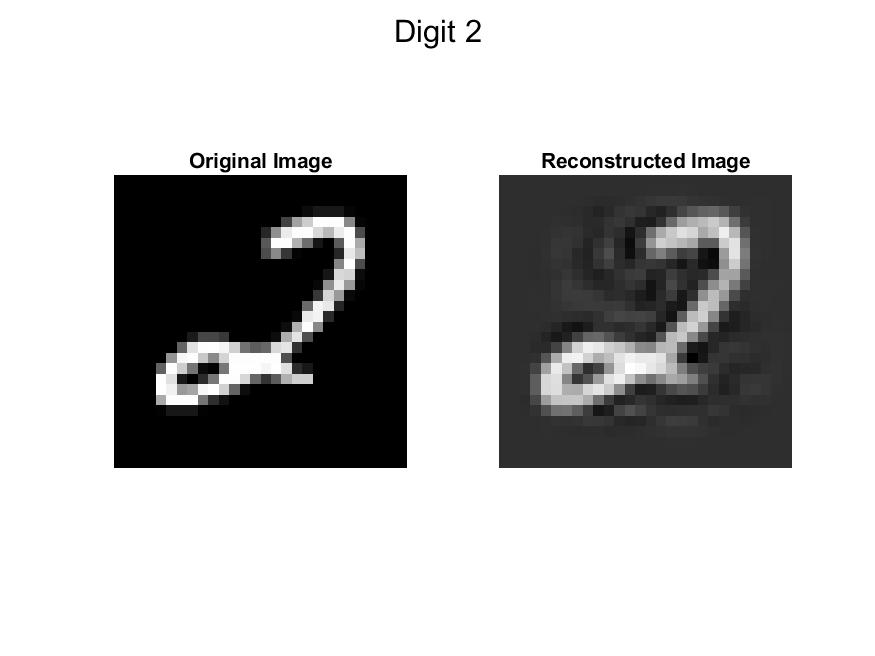
\includegraphics[height=0.40\textwidth]{q5/comp_2.jpg}}
        \ffigbox[0.47\textwidth]{}
        {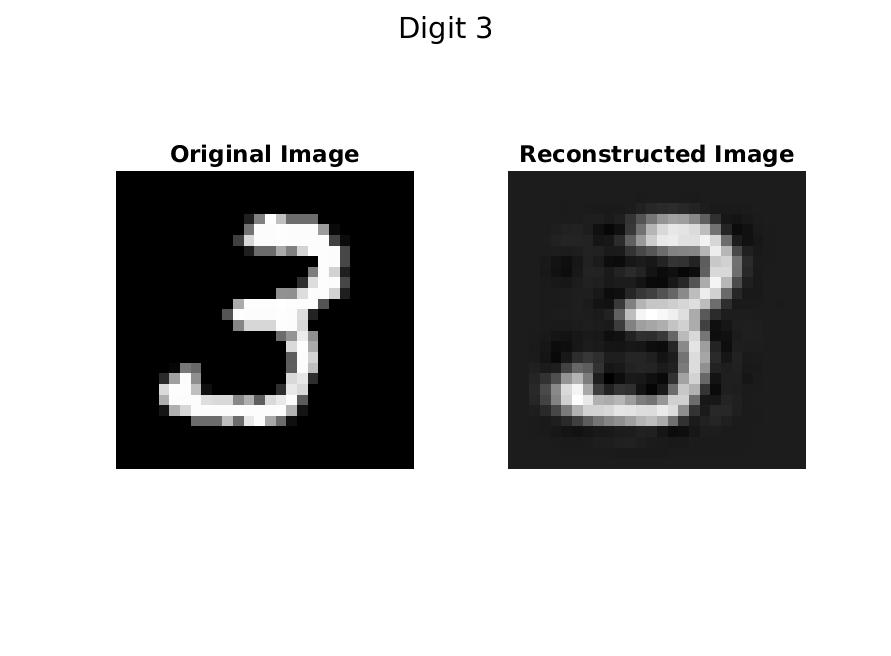
\includegraphics[height=0.40\textwidth]{q5/comp_3.jpg}}
    \end{floatrow}
\end{figure}
\begin{figure}[H]
    \begin{floatrow}
        \ffigbox[0.47\textwidth]{}
        {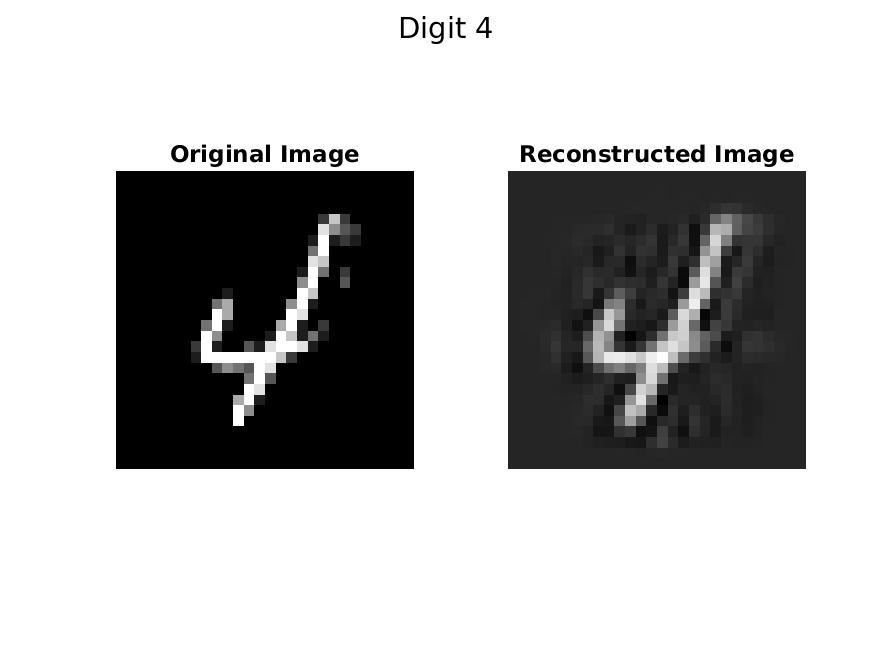
\includegraphics[height=0.40\textwidth]{q5/comp_4.jpg}}
        \ffigbox[0.47\textwidth]{}
        {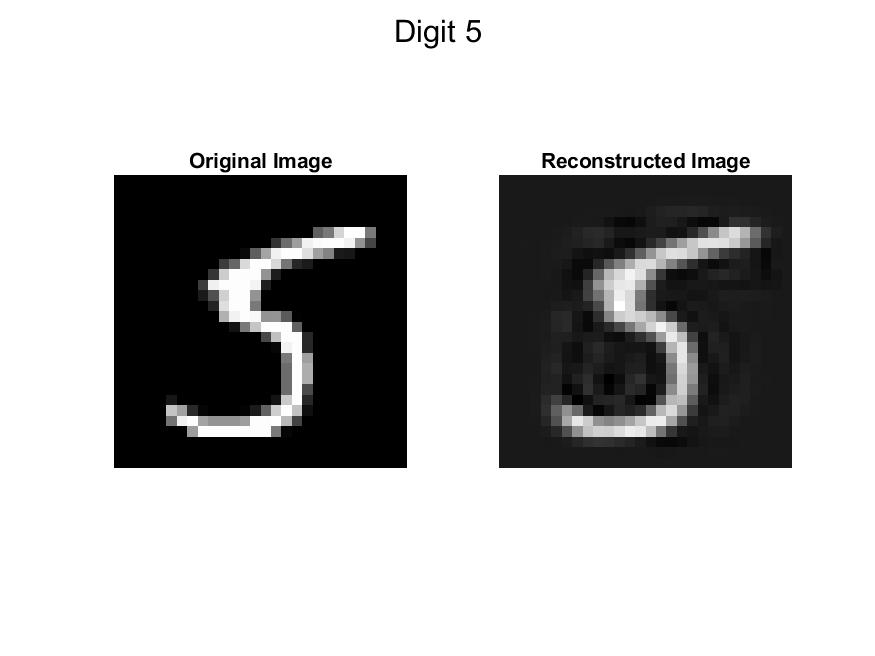
\includegraphics[height=0.40\textwidth]{q5/comp_5.jpg}}
    \end{floatrow}
\end{figure}
\begin{figure}[H]
    \begin{floatrow}
        \ffigbox[0.47\textwidth]{}
        {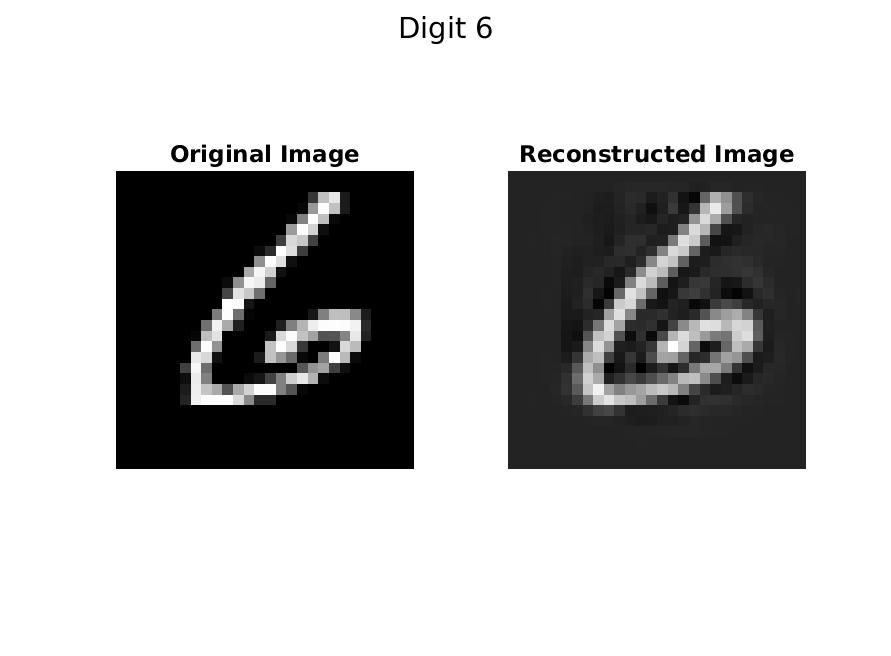
\includegraphics[height=0.40\textwidth]{q5/comp_6.jpg}}
        \ffigbox[0.47\textwidth]{}
        {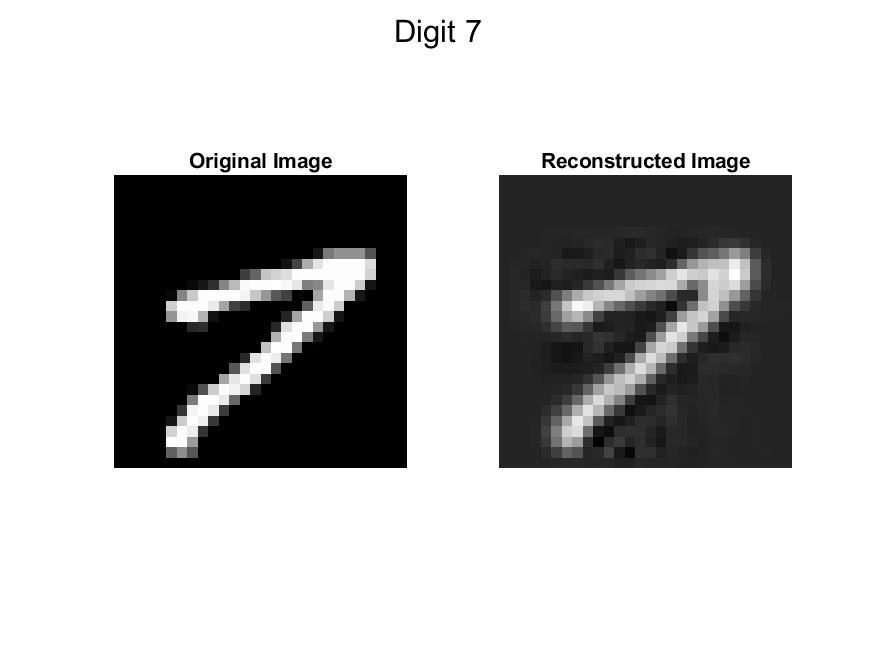
\includegraphics[height=0.40\textwidth]{q5/comp_7.jpg}}
    \end{floatrow}
\end{figure}
\begin{figure}[H]
    \begin{floatrow}
        \ffigbox[0.47\textwidth]{}
        {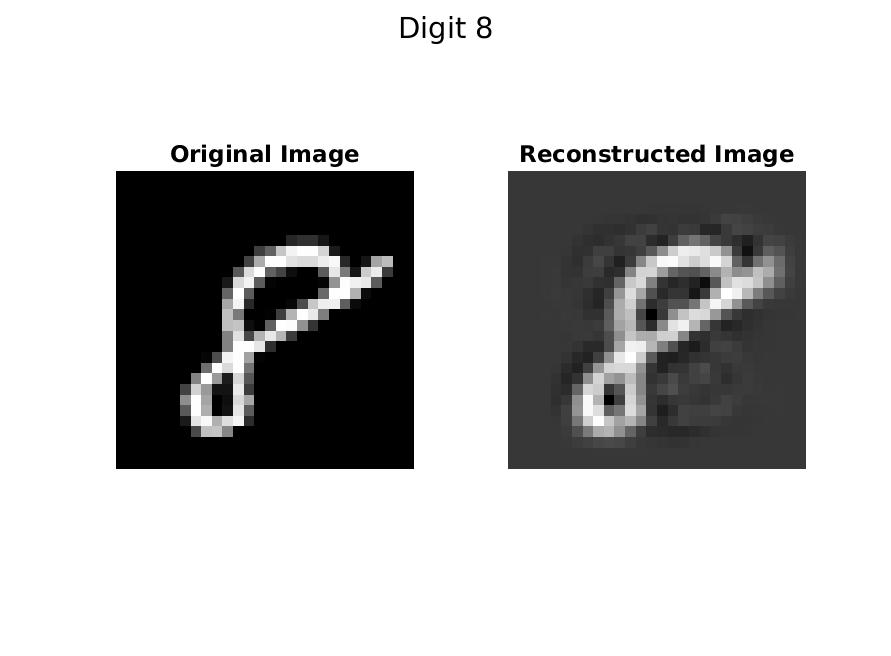
\includegraphics[height=0.40\textwidth]{q5/comp_8.jpg}}
        \ffigbox[0.47\textwidth]{}
        {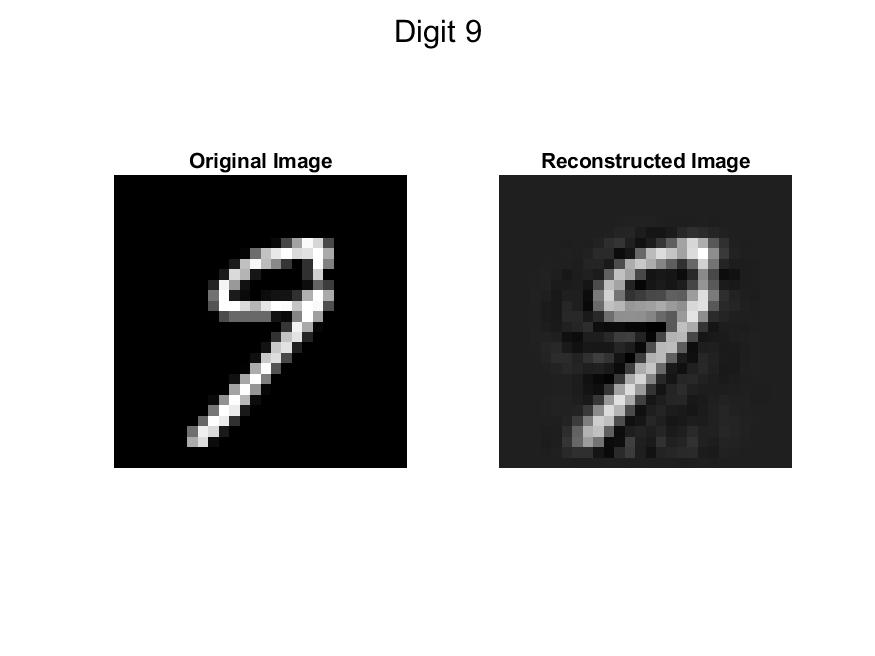
\includegraphics[height=0.40\textwidth]{q5/comp_9.jpg}}
    \end{floatrow}
\end{figure}

\newpage
\section*{Question 6}
\addcontentsline{toc}{section}{Question 6}
\setcounter{equation}{0}
\setcounter{figure}{0}
\subsection*{Closest Representation:}
Let $d = 80\times80\times3$\\
Let the sample mean of the original data be $\mu \in \mathbb{R}^d$, the sample covariance matrix of the original data be $C \in \mathbb{R}^{d\times d}$\\
Let the 4 chosen (normalized) eigenvectors of $C$ be $e_1, e_2, e_3, e_4 \in \mathbb{R}^d$\\ 
Let the original images (uncentered) be $\{x_i\}_{i=1}^N$, in this case $N = 16$\\
Then, the projection of $x_i$ onto the new dimensions will be given by $\sum_{j=1}^{4}((x_i - \mu)\cdot e_j)e_j$.\\
Now, since the projections are in a mean centered space, to come back into the uncentred space, we need to add $\mu$ to get the reconstruction of the original image:
$$
    \boxed{r_i = \mu + \sum_{j=1}^{4}((x_i - \mu)\cdot e_j)e_j}
$$
Thus, the coefficients used in the linear combination are $\boxed{c_{ij} = (x_i - \mu)\cdot e_j}$, now we need to prove that these coefficients indeed minimize the frobenius norm, which is equivalent to minimizing the square of the frobenius norm.\\

For the $i^{th}$ unrolled image, square of the frobinius norm is given by:
$$ 
    f_i^2 = ||x_i - r_i||^2 
$$

Note that $x_i$ is \textbf{exactly} equal to $ \mu + \sum_{j=1}^{d}((x_i - \mu)\cdot e_j)e_j $ (Sum of projections over \textbf{all} the eigenvectors of $C$), thus:
$$
\begin{aligned}
    f_i^2 &= \left|\left|\mu + \sum_{j=1}^{d}((x_i - \mu)\cdot e_j)e_j - (\mu + \sum_{j=1}^{4}((x_i - \mu)\cdot e_j)e_j)\right|\right|^2 \\
    &= \left|\left|\sum_{j=1}^{d}((x_i - \mu)\cdot e_j)e_j - \sum_{j=1}^{4}((x_i - \mu)\cdot e_j)e_j\right|\right|^2\\
    &= \left|\left|\sum_{j=5}^{d}((x_i - \mu)\cdot e_j)e_j\right|\right|^2 = \left|\left|\sum_{j=5}^{d}c_{ij}e_j\right|\right|^2\\
    &\text{Since any pair of $e_j$s are orthogonal, and $e_j$ are unit vectors,}\\
    f_i^2 &= \left|\left|\sum_{j=5}^{d}c_{ij}e_j\right|\right|^2 = \sum_{j=5}^{d}c_{ij}^2 = \sum_{j=5}^{d}((x_i - \mu)\cdot e_j)^2\\ 
\end{aligned}
$$
Thus we need to \textbf{minimize} $ \sum_{j=5}^{d}((x_i - \mu)\cdot e_j)^2$\\
Now, the variance of the projected data which PCA \textbf{maximizes} is $\sum_{j=1}^{4}((x_i - \mu)\cdot e_j)^2$\\
Since, 
$$ 
\begin{aligned}
    x_i &= \mu + \sum_{j=1}^{d}((x_i - \mu)\cdot e_j)e_j\\ 
    (x_i - \mu)^2 &= (\sum_{j=1}^{d}((x_i - \mu)\cdot e_j)e_j)^2 \\
    &\text{Since any pair of $e_j$s are orthogonal, and $e_j$ are unit vectors,}\\
    &= \sum_{j=1}^{d}((x_i - \mu)\cdot e_j)^2 = \sum_{j=1}^{4}((x_i - \mu)\cdot e_j)^2 + \sum_{j=5}^{d}((x_i - \mu)\cdot e_j)^2\\
    \Aboxed{(x_i - \mu)^2 &= constant =  \sum_{j=1}^{4}((x_i - \mu)\cdot e_j)^2 + \sum_{j=5}^{d}((x_i - \mu)\cdot e_j)^2} 
\end{aligned}
$$
Thus, \textbf{maximizing} the variance of the projected data: $\sum_{j=1}^{4}((x_i - \mu)\cdot e_j)^2$ is same as \textbf{minimizing} the frobenius norm of the difference: $\sum_{j=5}^{d}((x_i - \mu)\cdot e_j)^2 = f_i^2 $.
 
\medskip
Thus, in effect, PCA minimizes the frobenius norm of the difference between the projected and the actual image.\\
We follow the same way to reconstruct the images in our algorithm.\\
Let $E = [e_1\  e_2\  e_3 \ e_4]^T \in \mathbb{R}^{d \times 4} $, let $X \in \mathbb{R}^{d \times 16}$ contain the mean centered data, then $A = X^TE \in \mathbb{R}^{16 \times 4}$, where $A_{ij} = c_{ij}$, and thus the reconstructed data $\hat X = \mu + EA^T \in \mathbb{R}^{d \times 16}$, here $\mu$ is added to each column of $EA^T$.\\
In MATLAB:
\begin{verbatim}
    % data is the mean centered data 
    % Q4 contains the 4 eigenvectors, coeffs contain the required coefficients 
    coeffs = data' * Q4; % 16x4
    data_reconstructed = mu + Q4*coeffs';
\end{verbatim}

\subsection*{Generating new images:}
For generating new images, we need to sample data in the reduced domain and then project it back into the original domain.\\
In the projected domain, each point looks like $\mathbf{c} = [c_1\  c_2\  c_3\  c_4]^T \in \mathbb{R}^4$, to project this back into the original domain ($\mathbb{R}^d$):
$$
\begin{aligned}
    x_{gen} &= \mu + \sum_{j=1}^{4}c_j\mathbf{e_j}\\
\end{aligned}
$$
Thus, we need to sample $\mathbf{c}$.\\
We assume that $c \thicksim \mathcal{N}(\mathbf{0}, C)$ (A 0-mean multivariate gaussian with covariance matrix $C \in \mathbb{R}^{4\times 4}$)\\
We take $C = diag([\lambda_1, \lambda_2, \lambda_3, \lambda_4])$, since the variance of the original data along the chosen eigenvectors is given by the corresponding eigenvalues.\\
Now we sample random vectors $\mathbf{c}$ from this multivariate gaussian, project back to the original space and plot the images.\\
We achieve the following results which are different, but representative of the dataset:

\end{document}
